\documentclass[a4paper]{article}
\usepackage[a4paper]{geometry}
\usepackage{makeidx}
%\usepackage{fullpage}
\usepackage{graphicx,float}
\usepackage{t1enc}
%\usepackage{pdfsync}
\usepackage[latin1]{inputenc}
\usepackage{mathrsfs,xspace}
\usepackage{bm,amsmath,amssymb}
%\usepackage[show]{chato-notes}
%\usepackage{textcomp}
%\usepackage{tikz}
\usepackage{algorithmic}
\usepackage[normalsize]{subfigure}
\usepackage{sidecap}
\usepackage{todonotes}

\usepackage{tikz}
\usetikzlibrary{arrows, chains, fit, quotes}

\usetikzlibrary{decorations.pathmorphing}
\usetikzlibrary{calc}
\usepackage{xcolor}

\colorlet{lgray}{gray!50}
\colorlet{dgray}{gray!80}

\newcounter{noqed}
\newcommand{\qed}{ \ifmmode\mbox{
}\fi\rule[-.05em]{.3em}{.7em}\setcounter{noqed}{0}}
\newenvironment{proof}[1][{}]{\noindent{\bf Proof#1.
}\setcounter{noqed}{1}}{\ifnum\value{noqed}=1\qed\fi\par\medskip}
%\advance\textheight by 1cm
%\advance\topmargin -0.2cm 

\newtheorem{lemma}{Lemma}
\newtheorem{definition}{Definition}
\newtheorem{theorem}{Theorem}

%\advance\textwidth by 2cm
%\advance\oddsidemargin by -1cm
%\advance\evensidemargin by -1cm

%\newcommand{\captionfonts}{\small}

\floatstyle{ruled}
\newfloat{Algorithm}{htpb}{alg}

\newcommand{\exit}[1]{\operatorname{exit}(#1)}
\newcommand{\parex}[1]{\operatorname{parex}(#1)}
\newcommand{\lcp}{\operatorname{lcp}}

\newcommand{\T}{\operatorname{T}}
\newcommand{\BT}{\operatorname{BT}}
\newcommand{\HT}{\operatorname{HT}}
\newcommand{\Q}{\mathscr Q}
\newcommand{\E}{\mathscr E}
\newcommand{\gleq}{\sqsubseteq}
\newcommand{\gsup}{\sqcup}
\newcommand{\ginf}{\sqcap}
\newcommand{\gbsup}{\bigsqcup}
\newcommand{\gbinf}{\bigsqcap}
\newcommand{\?}{\mskip1.5mu}


\newcommand{\lst}[2]{${#1}_0$,~${#1}_1$, $\dots\,$,~${#1}_{#2}$}
\newcommand{\lstone}[2]{${#1}_1$,~${#1}_2$, $\dots\,$,~${#1}_{#2}$}
\newcommand{\lstp}[2]{${#1}_0+1$,~${#1}_1+1$, $\dots\,$,~${#1}_{#2-1}+1$}

\newcounter{prgline}
\newcommand{\pl}{\theprgline\addtocounter{prgline}{1}}

\newenvironment{renumerate}{\renewcommand{\theenumi}{(\roman{enumi})}\begin{enumerate}}{\end{enumerate}}



% \newcommand{\IF}{\text{\textbf{if}}\xspace}
% \newcommand{\BEGIN}{\text{\textbf{begin}}\xspace}
% \newcommand{\FOR}{\text{\textbf{for}}\xspace}
% \newcommand{\TO}{\text{\textbf{to}}\xspace}
% \newcommand{\END}{\text{\textbf{end}}\xspace}
% \newcommand{\DO}{\text{\textbf{do}}\xspace}
% \newcommand{\OD}{\text{\textbf{od}}\xspace}
% \newcommand{\TEST}{\text{\textbf{test}}\xspace}
% \newcommand{\THEN}{\text{\textbf{then}}\xspace}
% \newcommand{\ELSE}{\text{\textbf{else}}\xspace}
% \newcommand{\TRUE}{\text{\textbf{true}}\xspace}
% \newcommand{\FALSE}{\text{\textbf{false}}\xspace}
% \newcommand{\VAR}{\text{\textbf{var}}\xspace}
% \newcommand{\CONST}{\text{\textbf{const}}\xspace}
% \newcommand{\RETURN}{\text{\textbf{return}}\xspace}
% \newcommand{\ARRAY}{\text{\textbf{array}}\xspace}
% \newcommand{\ZERO}{\text{\textbf{zero}}\xspace}
% \newcommand{\INC}{\text{\textbf{inc}}\xspace}
% \newcommand{\DEC}{\text{\textbf{dec}}\xspace}
% \newcommand{\LOR}{\text{\textbf{or}}\xspace}
% \newcommand{\LAND}{\text{\textbf{and}}\xspace}
% \newcommand{\OF}{\text{\textbf{of}}\xspace}
% \newcommand{\WHILE}{\text{\textbf{while}}\xspace}
% \newcommand{\SET}{\text{\textbf{set}}\xspace}
% \newcommand{\BOOLEAN}{\text{\textbf{boolean}}\xspace}
% \newcommand{\PROC}{\text{\textbf{procedure}}\xspace}
% \newcommand{\GOTO}{\text{\textbf{goto}}\xspace}
% \newcommand{\STOP}{\text{\textbf{stop}}\xspace}
% \newcommand{\SUCC}{\text{succ}}
% \newcommand{\NULL}{\text{\textbf{null}}\xspace}
% \newcommand{\FUNCTION}{\text{\textbf{function}}\xspace}
% \newcommand{\PROCEDURE}{\text{\textbf{procedure}}\xspace}
% \newcommand{\var}[1]{{\itshape #1}}

\providecommand{\comp}{\circ}

\newcommand{\lb}{LB}
\newcommand{\rb}{RB}

\newcommand{\rank}{\operatorname{rank}}
\newcommand{\bucket}{\operatorname{bucket}}
\newcommand{\cnt}{\operatorname{count}}
\newcommand{\select}{\operatorname{select}}
\newcommand{\lgl}{\lceil\lg\ell\rceil}
\newcommand{\sing}[1]{\{\!#1\!\}}
\newcommand{\lsem}{\mathopen{[\![}}
\newcommand{\rsem}{\mathclose{]\!]}}
\newcommand{\sat}[2]{\lsem #2 \rsem_{#1}}

\def\..{\,\mathpunct{\ldotp\ldotp}} % Middle stuff for intervals. Usage: \..

\newcommand{\ebsuff}{\trianglelefteq}
\newcommand{\rmore}{\trianglerighteq}
\newcommand{\sbprol}{\preceq}
\newcommand{\sbprolneq}{\prec}
\newcommand{\kw}[1]{\textbf{#1}}

\newcommand{\I}{\mathscr I}
\newcommand{\C}{\mathscr C}
\newcommand{\A}{\mathscr A}
\newcommand{\op}{{\operatorname{op}}}
\newcommand{\url}{\cite{myurl}}


\renewcommand{\emptyset}{\varnothing}
\renewcommand{\epsilon}{\varepsilon}
\renewcommand{\phi}{\varphi}

% \numberofauthors{3}
% \title{Monotone Minimal Perfect Hashing}
% \subtitle{Indexing a Sorted Table in Sublinear Space}
% \author{\alignauthor
% Djamal Belazzougui\\
% \affaddr{
% Institut National d'Informatique\\
% Oued Smar, Algiers, Algeria}\\
% \email{\normalsize\sffamily djamal.belazzougui@gmail.com}\\
% \alignauthor
% Paolo Boldi \\
% \affaddr{Universit\`a degli Studi di Milano, Italy}\\
% \email{\normalsize\sffamily boldi@dsi.unimi.it}\\
% \and
% \alignauthor Rasmus Pagh \\ 
% \affaddr{IT University of Copenhagen, Denmark}\\
% \email{\normalsize\sffamily pagh@itu.dk}\\
% \alignauthor Sebastiano
% Vigna\\
% \affaddr{Universit\`a degli Studi di Milano, Italy}\\
% \email{\normalsize\sffamily vigna@acm.org}\\
% }

\title{Z-Fast Tries}
\author{Djamal Belazzougui \and Paolo Boldi\and
Sebastiano Vigna}
\date{}


\begin{document}

\maketitle
\thispagestyle{empty}

\bibliographystyle{abbrv}

\begin{abstract}
We describe the \emph{z-fast trie}, a
data structure inspired by the research started by the van Emde Boas
trees~\cite{EKZDIEPQ} and followed by the development of x-fast tries and y-fast tries~\cite{WilLLWRQ}. 
Z-fast tries are very
simple, uniform data structures: given a set $S$ of $n$ variable-length prefix-free strings, a z-fast trie is
defined by a standard compacted trie on $S$ endowed with a dictionary of
size $n-1$. With this simple setup, the z-fast trie can enumerate keys
in sorted order and can perform the lookup of $x$
in time $O(\lg|x|)$, while updates are performed within the
same bounds in expectation (or with high probability using an appropriate
dictionary). We also show a simple modification that makes it
possible to handle strings of length at most $2^w$; in this case, lookups
and updates are supported in $O(|x|/w + \lg|x|)$ time 
(and $O(|x|/B + \lg|x|)$ I/Os in the cache-oblivious
model) with high probability. Finally, just adding two suitable pointers
per node, the z-fast trie can answer
predecessors/successors queries in time
$O(\lg\max\{\?|x|,|x^+|,|x^-|\?\})$ ($x^\pm$ is the
successor/predecessor of $x$ in $S$) for a string $x$ of length linear in the
machine-word size $w$. Prefix queries are answered in time $O(\lg|x|+k)$, and range queries in time
$O(\lg\max\{\?|x|,|y|,|x^-|,|y^+|\?\}+k)$, where $k$ is the number of elements
in the output and  $x$ (and $y$) represent the input of the
prefix (range) queries. In the case of strings 
of length at most $2^w$, predecessor/successor queries
and updates are supported in $O(|x|/w + \lg\max\{\?|x|,|x^+|,|x^-|\?\})$ time, 
(and $O(|x|/B + \lg\max\{\?|x|,|x^+|,|x^-|\?\})$ I/Os in the cache-oblivious
model) with high probability.
%  The space occupied
% by a z-fast trie, besides that necessary to store $S$, is just of $12n$
% pointers, $2n$ integers and, in the ``long string'' case, $O(n)$ signatures of
% $O(w)$ bits each.
\todo[inline]{Double-check the bounds}

\end{abstract}
% Leaf: pointer to key, pointer to node holding the key, left/right pointers
% Internal: left/right pointers, left/right jump pointers, pointer to leaf
% holding the key, parent extent length
% Dictionary: 2 signatures, 2 pointers.

\section{Introduction}

Data structures providing successor and predecessor primitives on strings are
usually classified into \emph{comparison-based} and \emph{digital} structures. The former
assume to be able to compare strings in constant time; the latter rely on the
actual (binary) digits forming the strings to do their job. Currently, the
comparison-based data structure of choice are balanced binary trees and the B-trees (or B$^+$-trees), whereas
digital structures have been object of a growing interest in the last years
starting from the introduction of van Emde Boas trees~\cite{EKZDIEPQ} and
fusion trees~\cite{FrWSITBFT}, which provide asymptotically faster alternatives
for large collections.

In this paper, we revisit the classical dynamic predecessor/successors problems on a
set $S$ of size $n$ from a universe of strings of length $\ell$. The static
version of this problem has been completely solved, with matching upper and
lower bounds~\cite{PaTRDNHSP}. If only linear space is available, in a significant
number of cases variants of the van Emde Boas tree~\cite{EKZDIEPQ} that answer in time $O(\lg\ell)$ are
optimal even in the static setting using randomization. Among such variants we
quote Willard's \emph{y-fast trie} and Mehlhorn and N\"aher's
structure~\cite{MeNBOD}, which uses dynamic perfect hashing~\cite{DKMDPHULB}. 

These two solutions are both two-level data structures using buckets;
within each bucket some other standard data structure is used to answer queries. This
approach makes these structures complicated, and makes it difficult to
decouple the space that is necessary to store the structure and the set $S$.
This is not only a practical issue when we are interested in sets of ``long''
strings (i.e., of length at most $2^w$, rather than $O(w)$, where $w$ is the
machine word) of variable length. 

% SEBA: remove?
%Moreover, the bounds for modifying the
%structure are amortised, as once in a while the structure of the buckets
%undergoes major modifications.

The data structure discussed in this paper, the \emph{z-fast trie}, can
be thought of as the first simple optimal digital data structure that is neither
recursive nor needs to use bucketing to achieve optimal time and linear space.
Moreover, we present a simple variant that provides results with high
probability within the same bounds of the standard version for ``long'' strings, always
using a number of words linear in $n$ (rather than in the number of bits that is
necessary to represent $S$). In both cases, our space estimates are \emph{not}
asymptotic: we can provide \emph{exact} bounds, which amount to about a dozen
machine words per element.

The name ``z-fast trie'' was used for the first time in~\cite{BBPMMPH}.
The structure described in this paper is inspired by the idea of \emph{fat
binary search} introduced therein, but has little else in common. In particular,
the structure described in~\cite{BBPMMPH} is a static structure that just
manipulates strings and returns strings: more precisely, it is only able to provide
the longest \emph{extent}~(see Section~\ref{sec:notation}) in the compacted trie
on $S$ that is a prefix of a given query string. The z-fast trie described
in this paper, instead, is
based on a standard compacted trie endowed with a dictionary, the \emph{z-map},
inspired by the static case, which makes it possible to locate quickly a string
using a variant of fat binary search. With respect to a standard compacted trie, moreover, each node contains two additional
pointers: on leaves, the additional pointers are used to keep track of the original set (as 
a doubly linked list); on internal nodes, the pointers make it possible to move
quickly to the farthest left/right descendant.

The z-fast trie can answer
optimally a number of other queries, such as predecessor/successor queries, prefix queries, and range queries.
The main combinatorial results we prove (Theorem~\ref{th:parex}
and~\ref{th:fatanc}) 
highlight a deep connection between jump pointers and fat
binary search that make it possible to update the additional pointers quickly.

\noindent\textbf{Results.} Given a prefix-free set $S$ of $n$ binary
strings, we let
\begin{align*}
	x^- &= \max\{\?y \in S \mid y< x\?\} &&\text{(the \emph{predecessor} of
	$x$ in $S$)}\\
	x^+ &= \min\{\?y \in S \mid y\geq x\?\} && \text{(the \emph{successor} of
	$x$ in $S$)},
\end{align*}
where $\leq$ is the lexicographic order. A \emph{predecessor/successor query} is
given by a string $x$, and the answer is $x^\pm$. An \emph{existential prefix
query} asks whether there are strings in $S$ with given prefix $x$. An
\emph{existential range query} is given by a pair $x$, $y$ of strings, and asks
whether there are strings in $S$ in the (lexicographic) interval $[x\..y)$.
Standard prefix (range, respectively) queries report the set of strings
(expressed as pointers) with prefix $x$ in $S$ (the set of strings in the
interval $[x\..y)$, respectively).

We work in the standard RAM model with a word of length $w$, allowing
multiplications\todo{Seba: Do we really need multiplications? Apparently they were useful only to get constant-time MSB computation.}, under a full randomness assumption\footnote{We remark that hash functions 
are only used to implement a hash table and to compute signatures in the ``long
string'' case.}. We also discuss results in the \emph{cache-oblivious} model~\cite{FLPCOA}, which
analyses RAM algorithms in the I/O model using an ideal cache replacement
strategy.

We prove the following statements:
\begin{theorem}
\label{th:bounds}
If the string length is bounded by $O(w)$, the z-fast trie answers
predecessor and successor queries in time $O(\lg\max(|x|,|x^+|,|x^-|))$,
existential prefix queries in time $O(\lg|x|)$ and existential range queries in
time $O(\lg\max\{\?|x|,|y|\?\})$. The expected time required for  insertions and deletions is 
$O(\lg\max\{\?|x|,|x^+|,|x^-\?\})$. Besides the space 
required to store $S$, the z-fast trie needs $12n$ pointers and $n$ integers.
\end{theorem}
For long strings (i.e., strings of length more than linear in $w$, but still at most $2^w$) we can
provide a simple randomized variant of the structure, the \emph{signed z-fast
trie}:
\begin{theorem}
\label{th:boundslong}
If the string length is at most $2^w$, the signed z-fast trie
answers predecessor and successor queries in time
$O(|x|/w + \lg\max\{\?|x|,|x^+|,|x^-|\?\})$ and $O(|x|/B +
\lg\max\{\?|x|,|x^+|,|x^-|\?\})$ I/Os (in the cache-oblivious model) \emph{with
high probability}. Existential prefix queries are answered, always w.h.p., in time 
$O(|x|/w + \lg|x|)$ and $O(|x|/B + \lg|x|)$ I/Os.
Existential range queries are answered, always w.h.p., in time 
$O(\max\{\?|x|,|y|\?\}/w + \lg\max\{\?|x|,|y|\?\})$ and
$O(\max\{\?|x|,|y|\?\}/B + \lg\max\{\?|x|,|y|\?\})$ I/Os. Insertions and deletions are
performed in time $O(\lg\max\{\?|x|,|x^+|,|x^-|\?\})$, in expectation. 
Besides the space required to store
$S$, the signed z-fast trie needs $12n$ pointers, $n$ integers, and $3n$
signatures of $O(w)$ bits each.
\end{theorem}
%We can also answer to prefix and range queries: if the answer is a set $A$
%whose elements are overall $t$ bits long, the additional time is
%$O(t/w  + \lg\max(|\min A|,|\max A|) + |A|)$ and the additional I/Os are
%$O(t/B + \lg\max(|\min A|,|\max A|) + |A|)$. We note that the $t/w$ and $t/B$ are
%unavoidable (they are necessary to write the output). 
We can also answer prefix and range queries: if the answer is a set of $k$ 
strings, then the I/O and time costs are the same as in the existential
case, plus $O(k)$ and $O(\lg\max\{\?|x^-|,|y^+|\?\} + k)$ for prefix and
range queries respectively. Note that the space bounds assume a worst-case dictionary 
using $3n$ buckets (e.g., a linear-probing hash table with load factor $2/3$ and 
backing arrays whose length is a power of two, or a variant of Cuckoo
hashing~\cite{PaRCH}). We remark that the only reason of having expectations in
the update bounds is the presence of a dictionary: improvements in
dynamic dictionaries reflects immediately in improvements to the z-fast trie
time and space bounds.

To our knowledge, this is the first paper to propose a digital data structure for
variable length strings with optimal performance in the RAM model and good
performance in the cache-oblivious model. Nonetheless, we stress the fact that
the main feature of z-fast tries is that they are simple data structures
which can be actually implemented, and that the space usage is just about a dozen
machine words per element, independently of the string length. A complete
implementation is distributed under the GNU Lesser General Public
License\footnote{\texttt{http://sux4j.dsi.unimi.it/}.}.

\noindent\textbf{Previous work.} \todo{This certainly needs to be updated.} From a RAM perspective, several structures
already provide optimal bounds both in terms of $n$ (e.g., Andersson and
Thorup~\cite{AnTDOSEST} achieve $O(\sqrt{\lg n/\lg\lg n})$ update/query
time) and in term of the string length for fixed-length strings (e.g., y-fast tries~\cite{WilLLWRQ}).
The main contribution of the z-fast trie is that it is a simple
structure that can be easily implemented, and that it works with variable-length strings
longer than $O(w)$.

Andersson and Thorup note that by using a trie on the alphabet $2^w$ and some
very careful bookkeeping it is possible to achieve $O(|x|/w + \sqrt{\lg
n/\lg\lg n})$ time by storing in each node of the trie a predecessor
structure.\footnote{Using other kinds of digital structures (e.g., the structure
described in this paper) it would be possible to achieve similarly
$O(|x|/w + \lg w)$, but this is of little advantage as $O(|x|/w+\lg
|x|)=(|x|/w+\lg(|x|/w)+\lg w)=O(|x|/w+\lg w)$.}
Although in principle this solution would be faster in the
RAM model than ours (for sufficiently small sets), in the
cache-oblivious model it would require $(|x|/w + \sqrt{\lg
n/\lg\lg n})$ I/Os---in most cases worse than $O(|x|/B
+\lg\max(|x|,|x^+|,|x^-|))$ I/Os achieved by our data structure. Moreover,
the construction is rather involved; finally, while the $O(|x|/w)$ term in our
bound is simply due to the evaluation of a hash function and some bit-vector
comparisons, the $O(|x|/w)$ term in the trie technique depends on $|x|/w$
accesses to dictionaries, an operation that in practice is orders of magnitude slower.

In the cache-oblivious model, the string B-trees and its
variants~\cite{FeGSBT} provide predecessor/successor queries using
$O(|x|/B+\lg_B n)$ I/Os. We remark that this bound is in general incomparable to ours. Finally, note
that the RAM time bound in this case is essentially always worse than ours.

\section{Notation and tools}
\label{sec:notation}

%In this section, we introduce some terminology and notation adopted throughout
%the rest of the paper. 
We use von Neumann's definition
and notation for natural numbers: for every natural number $n$, we let $n=\{\?0,1,\ldots,n-1\?\}$; 
hence $2=\{\?0,1\?\}$
and $2^*$ is the set of all binary strings.
If $x$ is a string, $|x|$ denotes its length, and $x$ juxtaposed with an interval is the substring of $x$ with
those indices (starting from 0, inclusive, and ending at $|x|$, exclusive). 
Thus, for instance, $x[a\..b)$
is the substring of $x$ starting at position $a$ (inclusive) and ending at position
$b$ (exclusive). We will write $x[a]$ for $x[a\..a]$. The symbol $\preceq$
denotes prefix order, and $\prec$ is its strict version. Following Knuth~\cite[7.1.3]{KnuACPIV} we use $\lambda x$ for
the index of the highest bit set, or most significant bit (i.e., $\lambda x = \lfloor \lg x \rfloor$; $\lambda x$ is undefined when $x\leq 0$).
Note the easy mnemonics: $\lambda x$ is the position of the \emph{leftmost} one.

\subsection{2-fatness}

One of the key definitions that we will use in this paper is the following:

\begin{definition}[2-fattest numbers] 
\label{def:twofattest}
The \emph{2-fattest number} of an interval
$[a\..b]$ of integers is the unique integer in $[a\..b]$ that is
divisible by the largest power of two, or equivalently, that has the largest
number of trailing zeroes in its binary representation. 
\end{definition}

We will in general use ``fat'' for numbers
divisible by large powers of two, and ``lean'' with the opposite meaning. We
remark that if $f$ is 2-fattest in $[a\..b]$, it is also 2-fattest in every
subinterval of $[a\..b]$ that contains $f$, and that zero is the 2-fattest
number in any interval containing it.

Let us briefly discuss how to obtain the 2-fattest number in $[a\..b]$ assuming $a\neq 0$ (otherwise, the 2-fattest is simply 0).
Since the 2-fattest number in an interval $[a\..b]$ (that is, the value $f \in [a\..b]$
with maximum number of trailing zeroes) can be $a$ itself, it is easier to think about searching
for $f$ in the half-open interval $(a-1\..b]$. Looking at the binary expansion of $a-1$ and $b$,
$a-1$ and $b$  will have a certain longest common prefix $\ell$ followed by 
two suffixes, $\bar a$ and $\bar b$, which start with a 0 and a 1, respectively; for example:

\begin{center}
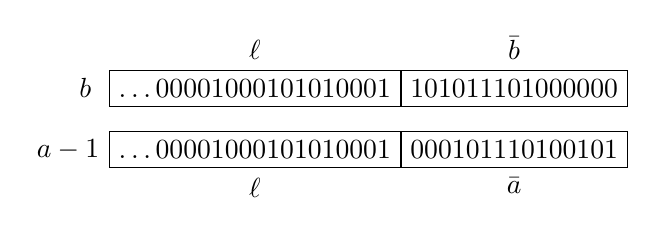
\begin{tikzpicture}
	\node (beq) {$b$};
	\node[rectangle, draw,label=above:$\ell$, right=1mm of beq] (lcpup) {$\dots00001000101010001$};
	\node[rectangle, draw,label=above:$\bar b$, right=0mm of lcpup, anchor=west] (bara)   {$101011101000000$};
	\node[rectangle, draw,label=below:$\ell$, below=3mm of lcpup] (lcpdown) {$\dots00001000101010001$};
	\node[rectangle, draw,label=below:$\bar a$, right=0mm of lcpdown] (barb) {$000101110100101$};
	\node[left=0mm of lcpdown] (aeq) {$a-1$};
\end{tikzpicture}
\end{center}
This first different bit between the two sequences is the most significant bit of
$(a-1) \oplus b$, and the 2-fattest number we are looking for is hence $(-1 \mathbin\ll \lambda((a-1) \oplus b)) \mathbin\& b$;
the final $\mathbin\& b$ brings in back the longest common prefix $\ell$:
\begin{center}
\begin{tikzpicture}
	\node (feq) {$f$};
	\node[rectangle, draw, right=1mm of beq] (lcp) {$\dots00001000101010001$};
	\node[rectangle, draw, right=0mm of lcp, anchor=west] (f)   {$100000000000000$};
\end{tikzpicture}
\end{center}

% Observe that finding the 2-fattest number in an interval $[a\..b]$ requires the computation of
% the most significant bit\footnote{More precisely, the 2-fattest number in
% $[a\..b]$ is $-1 \mathbin\ll \lambda(a-1 \oplus b) \mathbin\& b$.}, but
% alternatively we can check that $(-1\ll i)\mathbin\&(a-1) \neq (-1\ll i)\mathbin\&
% b$ for decreasing $i$: if the test is satisfied, the number is $b \mathbin\& -1
% \mathbin\ll i$, otherwise we decrement $i$.

\smallskip
We also introduce the following:

\begin{definition}[2-fat jump]
Given a positive integer $x$, the \emph{(2-fat) jump} of
$x$ is the smallest integer
$x'$ larger than $x$ having more trailing zeroes than $x$.  
Similarly, the \emph{(2-fat) backjump} of $x$ is the largest
integer smaller than $x$ with more trailing zeroes than $x$.
Formally, if $x=a2^b$ (with $a$ odd), then
\begin{eqnarray*}
	x'&=&(a+1)2^b\\
	x_\prime&=&(a-1)2^b. 
\end{eqnarray*}
Moreover, we let $0'=\infty$ and $0_\prime=0$.
We let $x^{(n)}$ ($x_{(n)}$, respectively) denote the application of $n$ jumps (backjumps, resp.),
that is $x^{(0)}=x$ and $x^{(n+1)}=\bigl(x^{(n)}\bigr)'$ ($x_{(0)}=x$ and $x_{(n+1)}=\bigl(x_{(n)}\bigr)_\prime$, resp.).
\end{definition}
For example, Fig.~\ref{fig:tablejumps} shows the jumps and backjumps of $88$.

\begin{figure}
\renewcommand{\arraystretch}{1.2}
\begin{tabular}{ccc}
\begin{tabular}{rrr}
Jump & Decimal value & Binary value\\\hline
$x^{(0)}$ & $88$ &     $1011000$\\
$x^{(1)}$ & $96$ &     $1100000$\\
$x^{(2)}$ & $128$ &   $10000000$\\
$x^{(3)}$ & $256$ &  $100000000$\\
$x^{(4)}$ & $512$ & $1000000000$\\
$\ldots$ & $\dots$ & $\ldots$
\end{tabular} & $\qquad$ &
\begin{tabular}{rrr}
Backjump & Decimal value & Binary value\\\hline
$x_{(0)}$ & $88$ & $1011000$\\
$x_{(1)}$ & $80$ & $1010000$\\
$x_{(2)}$ & $64$ & $1000000$\\
$x_{(3)}$ & $0$ & $0$\\
$x_{(4)}$ & $0$ & $0$\\
$\ldots$ & $\dots$ & $\ldots$
\end{tabular} 
\end{tabular}
\label{fig:tablejumps}\caption{2-fat jumps and backjumps of $x=88$.}
\end{figure}

Note that $(2^n)_\prime=0$, but $(2^n)'=2^{n+1}$. It is an easy observation that iterating $n$ times a jump we always obtain a
number larger than or equal to $2^n$ (i.e., $x^{(n)}\geq 2^n$ for all $x$ and $n$), and
ultimately the sequence of jumps of a positive number becomes a sequence of consecutive powers of 2.  
Conversely, for every $x>0$ there is some $n$ such that $x_{(n)}=0$.
These properties will be silently used throughout the paper.

We will need the following lemmata:
\begin{lemma}
\label{lemma:updown}
For every $x$, $x'\leq (x_\prime)'$ and $(x')_\prime \leq x_\prime$.
\end{lemma}
\begin{proof}
Let $x=a2^b$ with $a$ odd and $b\geq 0$. Then $x_\prime=(a-1)2^b$ and $x'=(a+1)2^b$. Since $a-1$ is even,
let $a-1=\bar a2^c$ for some $\bar a$ odd and $c>0$.
By contradiction, if 
\begin{eqnarray*}
(x_\prime)' &<& x'\\
(\bar a + 1)2^c2^b &<& (a+1)2^b\\
\bar a 2^c + 2^c &<& a+1\\
a-1+2^c &<& a+1\\
2^c &<& 2  
\end{eqnarray*}
contradicting the fact that $c>0$.
The other inequality follows similarly.\qed
\end{proof}

\begin{lemma}
\label{lemma:semipar}
If $x_\prime<y<x$ then $y'\leq x$.
\end{lemma}
\begin{proof}
Since $x_\prime$ is the largest number smaller than $x$ and 2-fatter than it, $y$ is either as fat as $x$,
or leaner. If $y$ is leaner, then clearly $y'\leq x$. If they are equally fat, say $y=a2^b$ and $x=\bar a2^b$,
for $a,\bar a$ odd, we have $y'=(a+1)2^b<\bar a2^b=x$.  \qed
\end{proof}

\begin{lemma}
\label{lemma:twofateq}
	Given a positive integer $r$, let $a_0=0$, and $a_{k+1}$ be the 2-fattest
	number in $[a_k+1\..r]$. Then
	$\{\?a_0,a_1,\dots,a_t=r\?\}=\{\?r_{(n)} \mid n \geq 0\?\}$.
	Morevoer, $t$ is equal to the number of ones in the binary expansion of $r$.
\end{lemma}
\begin{proof}
First note that $0$ belongs to both sets. Now let
$p_1>p_2>\dots>p_k$ be the positions of the ones in the binary expansion of $r$:
the $i$-th backjump of $r$ is exactly $r_{(i)}=\sum_{j\leq k-i}2^{p_j}$.
We prove that $a_i=r-r \bmod 2^{p_i}$ for all $i>0$. For $i=1$, $a_1$ is by definition the
2-fattest number in $[1\..r]$, which is exactly the largest power of two in such
interval. For the inductive step, we have defined $a_{i+1}$ as the 2-fattest
number in the interval $[r-r \bmod 2^{p_i}+1\..r]$; observing that $r=\sum_j
2^{p_j}$, we deduce that $a_{i+1}=r-r \bmod 2^{p_{i+1}}$. The thesis follows
easily.\qed
\end{proof}

\begin{lemma}[Parenthesis property]
\label{lemma:paren}
For positive integers $x$ and $y$ we have 
	that \[	x_\prime<y<x' \quad\implies\quad x_\prime\leq y_\prime < y'\leq x'.
	\]
\end{lemma}
\begin{proof}
By contradiction, suppose first that $x_\prime<y<x'<y'$, that is,
$(2h)2^b<(2k+1)2^c<(2h+2)2^b<(2k+2)2^c$, where $x=(2h+1)2^b$ and
$y=(2k+1)2^c$. If $b<c$, dividing by $2^{b+1}$ we obtain
$h < (2k+1)2^{c-(b+1)}<h+1$, which is impossible. Otherwise, if $b\geq c$
dividing by $2^c$ we obtain $2k+1<(2h+2)2^{b-c} < 2k+2$, which is again impossible. 
Reasoning analogously about $y_\prime<x_\prime<y<x'$ completes the
proof.\qed
% \noindent(Third item) Suppose that $y<x<y'$ and $z<x<z'$, and that $y=a2^b$,
% $z=c2^d$. The case $b=d$ is impossible, unless $y=z$; indeed, if $y\neq z$, say
% $y<z$, then $b=d$ would imply $a<c$ and hence $y'<z'$, so $y<z<y'<z'$, contradicting
% the parenthesis property; on the other hand $y=z$ would immediately imply $b=d$.
% In other words, for every $b\leq \lg x$ there is at most one $a$ such that
% $a2^b<x<(a+1)2^b$.
\end{proof}



\section{The simple z-fast trie} 

We start by describing the \emph{simple z-fast trie}, which is 
given by a compacted trie~\cite{KnuACP} endowed with a dictionary. 
More precisely, the simple z-fast trie can be
thought of as an indexing structure built on a set of prefix-free binary strings $S$
(stored somewhere in memory), and made of two components:
\begin{itemize}
  \item a compacted trie on the set $S$, whose nodes contain some ancillary data that will be described later;
  \item a dictionary, the \emph{z-map}, whose keys are binary
  strings and whose values are pointers to internal nodes of the trie.
\end{itemize}
% In the following section we are going
% to describe each component in detail and we will explain on how they are used at query time. 

The simple z-fast trie can answer membership queries, only, in time logarithmic in the key length, and it can enumerate its
keys in sorted order in linear time. While such a structure is of little interest,
describing the z-fast trie in steps highlights the modularity of the data structure
and should make it easier to understand the basic concepts.
In Section~\ref{sec:jumppointers} we will add 
two further pointers per node, making other types of query available.

\subsection{The compacted trie}
We start by defining some basic notation
that will be necessary to describe operations on the trie. Consider the compacted
trie $T(S)$~\cite{KnuACP} built for a prefix-free set of strings
$S\subseteq 2^*$. 
For any given node $\alpha$ of the
trie, we give the following definitions (see Figure~\ref{fig:ztrie}):
\begin{figure}[h!]
\centering
\includegraphics[scale=.9]{fig/prefix-1.mps}\qquad\raisebox{2cm}{\small
$Z$~\begin{tabular}{c}
\fbox{\begin{tabular}{lcl}
$\epsilon$& $\to$ & root\\
00100110 & $\to$ & $\alpha$\\
\end{tabular}}\qquad
\end{tabular}
}
\caption{\label{fig:ztrie}(above) A compacted trie for $\{\?001001010,0010011010010,00100110101\?\}$,
and the corresponding nomenclature and dictionary. The handles of the two internal nodes are delimited
by dashed lines. The example string $00100100$ exits on the left.}
\end{figure}
\begin{itemize}
    \item every internal node $\alpha$ has two children, called left child (or $0$-child)
    and right child (or $1$-child).
	\item $c_\alpha$, the \emph{compacted path of node $\alpha$}, is the string
	stored at $\alpha$;
	\item $n_\alpha$, the \emph{name of node $\alpha$}, is defined recursively as
	follows: the name of the root is $\epsilon$, and if $\alpha$ is the $t$-child
	of $\beta$ (where $t \in 2$), then $n_\alpha=n_\beta c_\beta  t$
	\item $e_\alpha$, the \emph{extent of node $\alpha$}, is defined as $e_\alpha=n_\alpha c_\alpha$;
	it is the longest common prefix of the strings represented by the leaves 
	that are descendants of $\alpha$; note that if $\alpha$ is the $t$-child
	of $\beta$ (where $t \in 2$), then $n_\alpha=e_\beta t$
	\item given a string $x$, we let $\exit x$ be the exit node of $x$, that is,
	the only node $\alpha$ such that $n_\alpha \preceq x$ and either $e_\alpha=x$ or $e_\alpha$
	is not a prefix of $x$; moreover, we call \emph{parex node of $x$} the
	\emph{parent} of the exit node of $x$, or a special symbol $\bot$ if the exit
	node of $x$ is the root (note that the parex of $x$ is the node with the
	longest extent that is a \emph{proper} prefix of $x$);
	\item the \emph{skip interval} $[i_\alpha\..j_\alpha]$ associated to
	$\alpha$ is $[|n_\alpha|\..|e_\alpha|]$ (note that the left extreme is
	$0$ for the root);
	\item we say that $x$ \emph{exits on the left} if $x \preceq e_{\exit x}$, or if $x$ and $e_{\exit x}$ 
	are $\preceq$-incomparable,
	and the first bit of $x$ after the longest common prefix with $e_{\exit x}$ is a 0; we say $x$ \emph{exits
	on the right} otherwise.
\end{itemize}

Every node $\alpha$ stores the extremes $i_\alpha$ and $j_\alpha$ of its skip interval, and its
own extent $e_\alpha$ (which is an element of $S$ on leaves); as usual, internal nodes contains two pointers to children.

\subsection{The z-map}

The z-map associates certain prefixes of the extents
of internal nodes, called \emph{handles}, with the corresponding node. This mapping
is sufficient to navigate the trie and find $\exit x$ in time $O(\lg|x|)$. The mapping is similar to that described in~\cite{BBPMMPH}, where
\emph{static probabilistic} z-fast tries were defined. Here we are going to prove some new important
properties of this mapping (in particular, its r\^ole in the discovery of
\emph{2-fat ancestors}). 

We start by associating with every node of the trie a string called its ``handle'':

\begin{definition}[handles] 
\label{def:twofattest}
The \emph{handle} $h_\alpha$ of a node $\alpha$ is the prefix of $e_\alpha$ whose length is 2-fattest number in the skip interval of $\alpha$
(see Figure~\ref{fig:ztrie}).
\end{definition}
Since zero is the 2-fattest number in every interval containing it, the handle of the root is always
the empty string $\varepsilon$.

\begin{definition}[z-map]
We define the map $Z$ from $2^*$ to the set of \emph{internal} nodes by
\[
Z:h_\alpha \mapsto \alpha,
\]
for every internal node $\alpha$.
\end{definition}
% We assume that $Z$ is actually implemented using a hash
% table, also denoted by $Z$, and that the entries of this hash table can also be 
% accessed (by their address) if needed
% (of course, any dictionary allowing satellite data will do the job).

We show an example of the handles of a z-fast trie over a small set of strings in Figure~\ref{fig:large-example}.


% A full discussion of the possible alternatives on how $Z$ is precisely
% implemented are deferred to a subsequent section.

\begin{figure}[htbp]
 \centering
 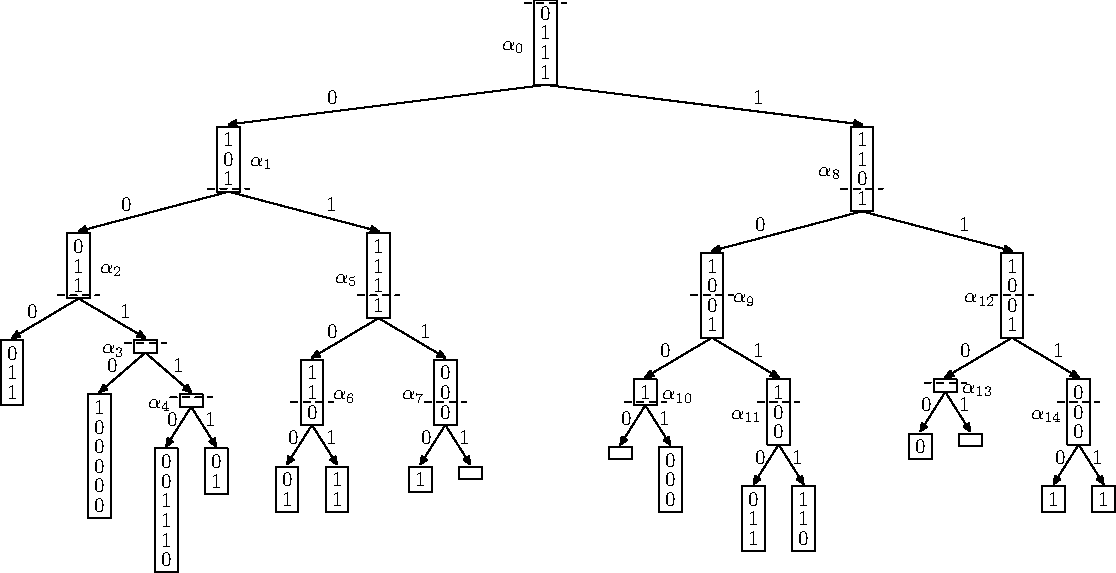
\includegraphics[scale=.6]{fig/large-example-1.pdf}
 \caption{\label{fig:large-example}The z-fast trie for a small set of strings. %$S=\{\,$01110101001110100000$, $01110101001110100011$, $01110101001111001101$, $01110101001111001110$, $01110101111110110001$, $01110101111110110111$, $01110101111111000010$, $01110101111111000111$, $01111110101001011000$, $01111110101001011010$, $01111110101001110000$, $01111110101001110010$, $01111110111001011100$, $01111110111001011101$, $01111110111001100001$, $01111110111001100011$\,\}$.
  The handles of internal nodes are delimited by dashed lines.}
\end{figure}


\begin{definition}[2-fat ancestors] Given a node $\alpha$, its \emph{2-fat
ancestors} are the nodes $\beta$ such that $h_\beta \in
\{\?e_\alpha[0\..|h_\alpha|_{(n)}) \mid n\geq 0\?\}$.
\end{definition}
The above definition may seem a bit cryptic: the idea is that we consider the
nodes on the path leading to $\alpha$ whose handle lengths are at least as fat
as $|h_\alpha|$. Note that not all handles in the definition above necessarily
exists, except for the last one, which is of course $\epsilon$---the handle of
the root.

2-fat ancestors will not be used in the simple z-fast trie, but they will be
essential in maintaining the additional pointers we will describe in Section~\ref{sec:jumppointers}.
To avoid duplication, we include their discovery in the algorithms that follows, even
if, technically, they are not needed in the case of simple z-fast tries. 


\subsection{Locating the parex node}

The most important property of $Z$ is that it makes us able to find very quickly
the parex node of a string and all of its 2-fat ancestors, using
the function LocateParex (Algorithm~\ref{algo:parex}):
in particular, at the end of the algorithm, on the top of the stack we will find
$\parex x$; if $x$ exits at the root, the algorithm will return an empty stack.



\begin{Algorithm}
\begin{algorithmic}
\STATE{\textbf{Function: } LocateParex}
\STATE{\textbf{Input:} a string $x$}
\STATE{\textbf{Output:} a stack containing the 2-fat ancestors of $\parex{x}$} 
\STATE $\Sigma\leftarrow\text{empty stack}$
\STATE $a, b\leftarrow 0,|x|$
\WHILE{$a \leq b$}
        \STATE{$f\leftarrow $ the 2-fattest number in $[a\..b]$}
        \STATE{$\beta\leftarrow Z(x[0\..f))$}
        \IF{$\beta\neq\bot$ \AND $e_\beta\prec x$} 
        	\STATE $a\leftarrow |e_\beta| + 1$ \COMMENT{Move from
        	$[a\..b]$ to 	$[|e_\beta|+1\..b]$} 
        	\STATE push $\beta$ on $\Sigma$
        \ELSE
           \STATE $b\leftarrow f - 1$ \COMMENT{Move from $[a\..b]$ to
           $[a\..f - 1]$}
        \ENDIF
\ENDWHILE
\STATE{{\bf return} $\Sigma$}
\end{algorithmic}
\caption{\label{algo:parex}At the end of the
execution, the stack contains $\parex x$ (on the top) and its
2-fat ancestors; if $x$ exits at the root, the algorithm returns the empty stack.}
\end{Algorithm}

Intuitively, Algorithm~\ref{algo:parex} works as follows: initially, it queries the Z-map
for the empty string, as $0$ is 2-fattest in all intervals, obtaining the root; afterwards, assuming $w$ \todo{Who is $w$, here? Should we say $w=|x|?$ and possibly use a different letter?} is a power of two,
it will query the Z-map with $x$, as now $w$ is the $2$-fattest number in $[1\..w]$, obtaining $\bot$, as leaves are not in the Z-map.
More interestingly, now Algorithm~\ref{algo:parex}  
 will query the Z-map with $x[0\.. w/2)$, the prefix of $x$ of length $w/2$.
 
Now, if there is a string in $S$ having $x[0\.. w/2)$ as prefix,
there must be a node $\alpha$ with an extent starting with $x[0\.. w/2)$: but $\alpha$ has necessarily $x[0\.. w/2)$ as handle,
because $w/2$ is 2-fattest in any subinterval of $[1\..w-1]$ that contains it. We can now move to the interval $[|e_\alpha|+1\..w]$ and continue in the
same way.

If, however, there is no string in $S$  having $x[0\.. w/2)$ as prefix, we try again with
$[0\.. w/4)$.

To prove formally the correctness of Algorithm~\ref{algo:parex}, let us define the
\emph{cutpoint} for a string $x$ with respect to a trie as the length of the
longest common prefix between $x$ and $e_{\exit x}$ (the extent of its exit node). There are two cases: 
we say that $x$ \emph{cuts high}
if the cutpoint is strictly smaller than $|h_{\exit x}|$, \emph{cuts low}
otherwise. Note that only in the second case the handle of $\exit x$ is a prefix
of $x$. 


\begin{theorem}
\label{th:parex}
Let $x$ be a nonempty string, and 
$\eta=\parex x$.
Let 
$\alpha_0$,~$\alpha_1$, $\dots\,$,~${\alpha}_{t}=\eta$
be the sequence of 2-fat ancestors of $\eta$ (the emtpy sequence if $\eta=\bot$)\todo{We should say how they are ordered (``in increasing handle-length order'')}.
Let $[a\..b]$ be the interval maintained by 
  Algorithm~\ref{algo:parex}. After each iteration the following
  invariant is satisfied: $a=|e_{\alpha_j}|+1$ for some $j$ and $|h_\eta|\leq b$; moreover 
  all values $|e_{\alpha_j}|+1$ are attained by $a$
  (in order of increasing $j$) at some point of the execution.
\end{theorem}
\begin{proof}
Let $\sigma$ be the node such that $h_\sigma$ is the longest handle in $Z$ that is a prefix of $x$:
note that either $\sigma=\eta$ (if $x$ cuts high or $\exit x$ is a leaf), or $\sigma=\exit x$ and
it is one of the children of $\eta$.  

The first value of $f$ is necessarily zero, so at the first execution $\beta$ is the root node;
if $e_\beta\not\prec x$, the exit node is the root (and we proceed correctly because we set $b=-1$ and immediately
exit the loop, returning the emtpy stack); conversely, if $e_\beta\prec x$, the invariant is true at the end of the first iteration (we set $a=|e_{\mathrm{root}}|+1$),
and we correctly push the root on the stack (the root is a fat ancestor of every other node).

We now prove by induction that in the rest of execution the invariant is true.
At each step we pick the
$2$-fattest number $f\in[|e_{\alpha_i}|+1\..b]$, and change interval. Let
$\beta=Z(x[0\..f))$. We have three cases:
\begin{itemize}
  \item If $f\leq |h_\eta|$, $x[0\..f)$
  must be the handle of a node $\beta$, as $f$ is
  2-fattest in
  $[|e_{\alpha_i}|+1\..b]\supseteq[|e_{\alpha_i}|+1\..|h_\eta|]$.
  Moreover, necessarily $\beta=\alpha_{i+1}$ because of Lemma~\ref{lemma:twofateq},
  and $e_\beta\prec x$ (because $\beta$ is an ancestor of $\eta=\parex x$). Thus, the algorithm sets
  $a=|e_\beta|+1=|e_{\alpha_{i+1}}|+1$ the invariant is preserved.
  \item If $|h_\sigma|<f$, necessarily 
  $\beta=\bot$. Thus, by setting $b=f-1\geq|h_\sigma|\geq |h_\eta|$  we
  preserve the invariant.
  \item The last case is when $|h_\eta|< f\leq |h_\sigma|$, which can only occur if $\sigma=\exit x$ is
  internal and $x$ cuts low. If $f$ belongs to the skip interval of $\eta$, we query $Z$ with something
  that is not a handle, so we get $\beta=\bot$. Otherwise, necessarily $f=h_\sigma$ hence we get $\beta=\sigma$ 
  but either $e_\sigma=x$ or $e_\sigma \not\preceq x$. In all cases, we set $b=f-1\geq |h_\eta|$
  and preserve the invariant.       
  \qed
\end{itemize}
\end{proof}

Table~\ref{tab:example-query-parex} shows an example of the execution of the algorithm. For each
execution of the loop, we show the current search interval $[a\..b]$, the 2-fattest number $f$,
the $\beta$ obtained by querying $Z$, whether $e_\beta\prec x$ or not (in the cases in which
$\beta\neq\bot$) and the stack after the execution of the iteration. 

\begin{table}
\centering
%\documentclass{article}
%\usepackage{tikz}
%\usetikzlibrary{arrows, chains, fit, quotes}

%\begin{document}
	{
	\setlength\tabcolsep{0.5em}
	\begin{tabular}{|l|r|r|r|c|c|c|}
	\hline
	& $a$ & $b$ & $f$ & $\beta$ & $e_\beta \prec x$? & Stack (after)\\\hline
	
	\rule{0pt}{2.5em}\rule[-2.5em]{0pt}{2.5em}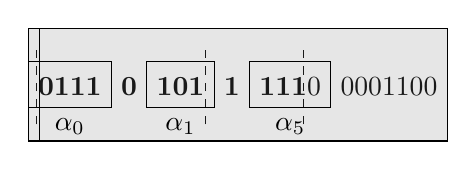
\begin{tikzpicture}[
	  baseline,
	  node distance = 0mm,
	  start chain = A going right,
	  txt/.style = {text height=2ex, text depth=0.25ex, 
	                 on chain},
	  every edge/.append style = {draw, -stealth'}
	  ]

	\node [txt] {$\mathbf{0111}$};     % nodes are in the chain
	\draw [dashed] ([xshift=3pt, yshift=-6pt]A-1.south west) -- ([xshift=3pt, yshift=6pt]A-1.north west);
	\node [txt] {$\mathbf{0}$};
	\node [txt] {$\mathbf{101}$};
	\draw [dashed] ([xshift=-3pt, yshift=-6pt]A-3.south east) -- ([xshift=-3pt, yshift=6pt]A-3.north east);
	\node [txt] {$\mathbf{1}$};
	\node [txt] {$\mathbf{111}0$};
	\draw [dashed] ([xshift=-10pt, yshift=-6pt]A-5.south east) -- ([xshift=-10pt, yshift=6pt]A-5.north east);
	\node [txt] {$0001100$};
	%
	\node (g) [draw=black, fill=black!50, fill opacity=0.2, inner ysep=12pt, inner xsep=0,
		   fit=(A-1) (A-6)] {};
	
	\node (f1)  [draw=black, inner sep=0pt, 
	             label=below:$\alpha_0$, 
	             fit=(A-1) (A-1)] {};
	\node (f3)  [draw=black, inner sep=0pt, 
	             label=below:$\alpha_1$,
	             fit=(A-3) (A-3)] {};

	\node (f5)  [draw=black, inner sep=0pt, 
	             label=below:$\alpha_5$,
	             fit=(A-5) (A-5)] {};

	\draw ([xshift=4pt, yshift=-12pt]A-1.south west) -- ([xshift=4pt, yshift=12pt]A-1.north west);
       \end{tikzpicture}
    & $0$ & $20$ & $0$ & $\alpha_0$ & yes & $\langle \alpha_0\rangle$\\\hline

    %%%%%%
	\rule{0pt}{2.5em}\rule[-2.5em]{0pt}{2.5em}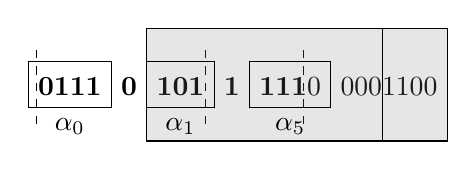
\begin{tikzpicture}[
	  baseline,
	  node distance = 0mm,
	  start chain = A going right,
	  txt/.style = {text height=2ex, text depth=0.25ex, 
	                 on chain},
	  every edge/.append style = {draw, -stealth'}
	  ]

	\node [txt] {$\mathbf{0111}$};     % nodes are in the chain
	\draw [dashed] ([xshift=3pt, yshift=-6pt]A-1.south west) -- ([xshift=3pt, yshift=6pt]A-1.north west);
	\node [txt] {$\mathbf{0}$};
	\node [txt] {$\mathbf{101}$};
	\draw [dashed] ([xshift=-3pt, yshift=-6pt]A-3.south east) -- ([xshift=-3pt, yshift=6pt]A-3.north east);
	\node [txt] {$\mathbf{1}$};
	\node [txt] {$\mathbf{111}0$};
	\draw [dashed] ([xshift=-10pt, yshift=-6pt]A-5.south east) -- ([xshift=-10pt, yshift=6pt]A-5.north east);
	\node [txt] {$0001100$};
	%
	\node (g) [draw=black, fill=black!50, fill opacity=0.2, inner ysep=12pt, inner xsep=0,
		   fit=(A-3) (A-6)] {};
	
	\node (f1)  [draw=black, inner sep=0pt, 
	             label=below:$\alpha_0$, 
	             fit=(A-1) (A-1)] {};
	\node (f3)  [draw=black, inner sep=0pt, 
	             label=below:$\alpha_1$,
	             fit=(A-3) (A-3)] {};

	\node (f5)  [draw=black, inner sep=0pt, 
	             label=below:$\alpha_5$,
	             fit=(A-5) (A-5)] {};

	\draw ([xshift=128pt, yshift=-12pt]A-1.south west) -- ([xshift=128pt, yshift=12pt]A-1.north west);
    \end{tikzpicture}
    & $5$ & $20$ & $16$ & $\bot$ & - & $\langle \alpha_0\rangle$\\\hline

    %%%%%%
	\rule{0pt}{2.5em}\rule[-2.5em]{0pt}{2.5em}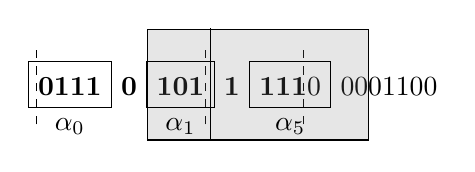
\begin{tikzpicture}[
	  baseline,
	  node distance = 0mm,
	  start chain = A going right,
	  txt/.style = {text height=2ex, text depth=0.25ex, 
	                 on chain},
	  every edge/.append style = {draw, -stealth'}
	  ]

	\node [txt] {$\mathbf{0111}$};     % nodes are in the chain
	\draw [dashed] ([xshift=3pt, yshift=-6pt]A-1.south west) -- ([xshift=3pt, yshift=6pt]A-1.north west);
	\node [txt] {$\mathbf{0}$};
	\node [txt] {$\mathbf{101}$};
	\draw [dashed] ([xshift=-3pt, yshift=-6pt]A-3.south east) -- ([xshift=-3pt, yshift=6pt]A-3.north east);
	\node [txt] {$\mathbf{1}$};
	\node [txt] {$\mathbf{111}0$};
	\draw [dashed] ([xshift=-10pt, yshift=-6pt]A-5.south east) -- ([xshift=-10pt, yshift=6pt]A-5.north east);
	\node [txt] {$0001100$};
	%
	\node (g) [draw=black, fill=black!50, fill opacity=0.2, inner ysep=12pt, inner xsep=0, minimum width=80pt, minimum height=40pt, anchor=west] at (A-3.west){};
	
	\node (f1)  [draw=black, inner sep=0pt, 
	             label=below:$\alpha_0$, 
	             fit=(A-1) (A-1)] {};
	\node (f3)  [draw=black, inner sep=0pt, 
	             label=below:$\alpha_1$,
	             fit=(A-3) (A-3)] {};

	\node (f5)  [draw=black, inner sep=0pt, 
	             label=below:$\alpha_5$,
	             fit=(A-5) (A-5)] {};

	\draw ([xshift=66pt, yshift=-12pt]A-1.south west) -- ([xshift=66pt, yshift=12pt]A-1.north west);
    \end{tikzpicture}
    & $5$ & $15$ & $8$ & $\alpha_1$ & yes & $\langle \alpha_0, \alpha_1\rangle$\\\hline

    %%%%%%
	\rule{0pt}{2.5em}\rule[-2.5em]{0pt}{2.5em}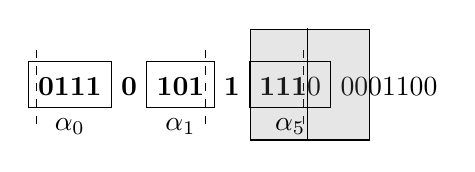
\begin{tikzpicture}[
	  baseline,
	  node distance = 0mm,
	  start chain = A going right,
	  txt/.style = {text height=2ex, text depth=0.25ex, 
	                 on chain},
	  every edge/.append style = {draw, -stealth'}
	  ]

	\node [txt] {$\mathbf{0111}$};     % nodes are in the chain
	\draw [dashed] ([xshift=3pt, yshift=-6pt]A-1.south west) -- ([xshift=3pt, yshift=6pt]A-1.north west);
	\node [txt] {$\mathbf{0}$};
	\node [txt] {$\mathbf{101}$};
	\draw [dashed] ([xshift=-3pt, yshift=-6pt]A-3.south east) -- ([xshift=-3pt, yshift=6pt]A-3.north east);
	\node [txt] {$\mathbf{1}$};
	\node [txt] {$\mathbf{111}0$};
	\draw [dashed] ([xshift=-10pt, yshift=-6pt]A-5.south east) -- ([xshift=-10pt, yshift=6pt]A-5.north east);
	\node [txt] {$0001100$};
	%
	\node (g) [draw=black, fill=black!50, fill opacity=0.2, inner ysep=12pt, inner xsep=0, minimum width=43pt, minimum height=40pt, anchor=west] at (A-5.west){};
	
	\node (f1)  [draw=black, inner sep=0pt, 
	             label=below:$\alpha_0$, 
	             fit=(A-1) (A-1)] {};
	\node (f3)  [draw=black, inner sep=0pt, 
	             label=below:$\alpha_1$,
	             fit=(A-3) (A-3)] {};

	\node (f5)  [draw=black, inner sep=0pt, 
	             label=below:$\alpha_5$,
	             fit=(A-5) (A-5)] {};

	\draw ([xshift=101pt, yshift=-12pt]A-1.south west) -- ([xshift=101pt, yshift=12pt]A-1.north west);
    \end{tikzpicture}
    & $9$ & $15$ & $12$ & $\alpha_5$ & no & $\langle \alpha_0, \alpha_1\rangle$\\\hline

    %%%%%%
	\rule{0pt}{2.5em}\rule[-2.5em]{0pt}{2.5em}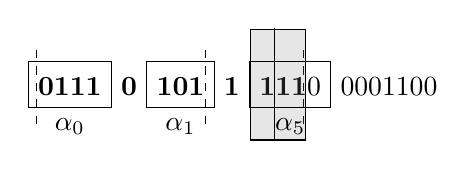
\begin{tikzpicture}[
	  baseline,
	  node distance = 0mm,
	  start chain = A going right,
	  txt/.style = {text height=2ex, text depth=0.25ex, 
	                 on chain},
	  every edge/.append style = {draw, -stealth'}
	  ]

	\node [txt] {$\mathbf{0111}$};     % nodes are in the chain
	\draw [dashed] ([xshift=3pt, yshift=-6pt]A-1.south west) -- ([xshift=3pt, yshift=6pt]A-1.north west);
	\node [txt] {$\mathbf{0}$};
	\node [txt] {$\mathbf{101}$};
	\draw [dashed] ([xshift=-3pt, yshift=-6pt]A-3.south east) -- ([xshift=-3pt, yshift=6pt]A-3.north east);
	\node [txt] {$\mathbf{1}$};
	\node [txt] {$\mathbf{111}0$};
	\draw [dashed] ([xshift=-10pt, yshift=-6pt]A-5.south east) -- ([xshift=-10pt, yshift=6pt]A-5.north east);
	\node [txt] {$0001100$};
	%
	\node (g) [draw=black, fill=black!50, fill opacity=0.2, inner ysep=12pt, inner xsep=0, minimum width=20pt, minimum height=40pt, anchor=west] at (A-5.west){};
	
	\node (f1)  [draw=black, inner sep=0pt, 
	             label=below:$\alpha_0$, 
	             fit=(A-1) (A-1)] {};
	\node (f3)  [draw=black, inner sep=0pt, 
	             label=below:$\alpha_1$,
	             fit=(A-3) (A-3)] {};

	\node (f5)  [draw=black, inner sep=0pt, 
	             label=below:$\alpha_5$,
	             fit=(A-5) (A-5)] {};

	\draw ([xshift=89pt, yshift=-12pt]A-1.south west) -- ([xshift=89pt, yshift=12pt]A-1.north west);
    \end{tikzpicture}
    & $9$ & $11$ & $10$ & $\bot$ & - & $\langle \alpha_0, \alpha_1\rangle$\\\hline

    %%%%%%
	\rule{0pt}{2.5em}\rule[-2.5em]{0pt}{2.5em}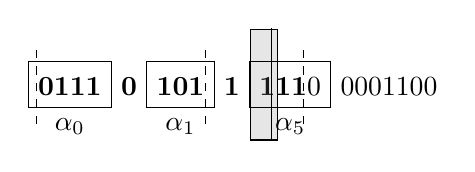
\begin{tikzpicture}[
	  baseline,
	  node distance = 0mm,
	  start chain = A going right,
	  txt/.style = {text height=2ex, text depth=0.25ex, 
	                 on chain},
	  every edge/.append style = {draw, -stealth'}
	  ]

	\node [txt] {$\mathbf{0111}$};     % nodes are in the chain
	\draw [dashed] ([xshift=3pt, yshift=-6pt]A-1.south west) -- ([xshift=3pt, yshift=6pt]A-1.north west);
	\node [txt] {$\mathbf{0}$};
	\node [txt] {$\mathbf{101}$};
	\draw [dashed] ([xshift=-3pt, yshift=-6pt]A-3.south east) -- ([xshift=-3pt, yshift=6pt]A-3.north east);
	\node [txt] {$\mathbf{1}$};
	\node [txt] {$\mathbf{111}0$};
	\draw [dashed] ([xshift=-10pt, yshift=-6pt]A-5.south east) -- ([xshift=-10pt, yshift=6pt]A-5.north east);
	\node [txt] {$0001100$};
	%
	\node (g) [draw=black, fill=black!50, fill opacity=0.2, inner ysep=12pt, inner xsep=0, minimum width=10pt, minimum height=40pt, anchor=west] at (A-5.west){};
	
	\node (f1)  [draw=black, inner sep=0pt, 
	             label=below:$\alpha_0$, 
	             fit=(A-1) (A-1)] {};
	\node (f3)  [draw=black, inner sep=0pt, 
	             label=below:$\alpha_1$,
	             fit=(A-3) (A-3)] {};

	\node (f5)  [draw=black, inner sep=0pt, 
	             label=below:$\alpha_5$,
	             fit=(A-5) (A-5)] {};

	\draw ([xshift=88pt, yshift=-12pt]A-1.south west) -- ([xshift=88pt, yshift=12pt]A-1.north west);
    \end{tikzpicture}
    & $9$ & $9$ & $9$ & $\bot$ & - & $\langle \alpha_0, \alpha_1\rangle$\\\hline

    %%%%%%
	\rule{0pt}{2.5em}\rule[-2.5em]{0pt}{2.5em}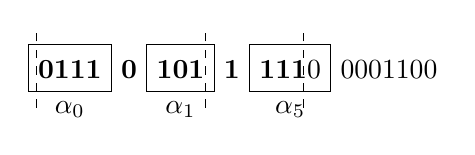
\begin{tikzpicture}[
	  baseline,
	  node distance = 0mm,
	  start chain = A going right,
	  txt/.style = {text height=2ex, text depth=0.25ex, 
	                 on chain},
	  every edge/.append style = {draw, -stealth'}
	  ]

	\node [txt] {$\mathbf{0111}$};     % nodes are in the chain
	\draw [dashed] ([xshift=3pt, yshift=-6pt]A-1.south west) -- ([xshift=3pt, yshift=6pt]A-1.north west);
	\node [txt] {$\mathbf{0}$};
	\node [txt] {$\mathbf{101}$};
	\draw [dashed] ([xshift=-3pt, yshift=-6pt]A-3.south east) -- ([xshift=-3pt, yshift=6pt]A-3.north east);
	\node [txt] {$\mathbf{1}$};
	\node [txt] {$\mathbf{111}0$};
	\draw [dashed] ([xshift=-10pt, yshift=-6pt]A-5.south east) -- ([xshift=-10pt, yshift=6pt]A-5.north east);
	\node [txt] {$0001100$};
	%
	\node (f1)  [draw=black, inner sep=0pt, 
	             label=below:$\alpha_0$, 
	             fit=(A-1) (A-1)] {};
	\node (f3)  [draw=black, inner sep=0pt, 
	             label=below:$\alpha_1$,
	             fit=(A-3) (A-3)] {};

	\node (f5)  [draw=black, inner sep=0pt, 
	             label=below:$\alpha_5$,
	             fit=(A-5) (A-5)] {};

    \end{tikzpicture}
    & $9$ & $8$ & - & - & - & $\langle \alpha_0, \alpha_1\rangle$\\\hline

    \end{tabular}
    }


%\end{document}

\vspace*{.5cm}
\caption{\label{tab:example-query-parex}Execution of Algorithm~\ref{algo:parex} on the trie of Figure~\ref{fig:large-example}
with $x=01110101111100001100$: the longest prefix of $x$ that is in the trie is in boldface (and
the corresponding nodes are used to label the frames). Here $\exit x=\alpha_5$ whereas $\parex x=\alpha_1$. 
The grey rectangle depicts the current search interval $[a\..b]$,
the vertical line indicates the position $f$, whereas the dashed lines refer to node handles.}
\end{table}

A few remarks are in order:
\begin{itemize}
  \item Algorithm~\ref{algo:parex} completes in at most $\lg|x|$ iterations.
  \item At the end of Algorithm~\ref{algo:parex}, the returned stack contains
  all and only the 2-fat ancestors of $\eta$ in increasing handle-length order (the empty
  stack if $\eta=\bot$).
  \item The exit node of $x$ can easily be recovered in constant
time from the output of Algorithm~\ref{algo:parex}:
if $\eta=\parex x$ then the exit node is the left or right child of $\eta$, depending on 
wheter $x[|e_\eta|]$ is a 0 or a 1.
  \item To perform deletions, we will need to compute the parent of the parex node: if it
  cannot be found on the stack just above the parex node, it can be computed by running
   Algorithm~\ref{algo:parex} on the name of the parex node (but see Section~\ref{sec:reusing} for an approach that is better in practice).
\end{itemize}

\subsection{Membership queries and updates}
\label{sec:updates}

Theorem~\ref{th:parex} implies that the simple z-fast trie achieves the bound of Theorem~\ref{th:bounds} for membership queries:
one can just locate the exit node of $x$ and check that it is a leaf and its extent is equal to $x$. We now discuss how to perform updates.

To insert a new string $x$ into the z-fast trie, we first locate the parex and
exit node of $x$ using Algorithm~\ref{algo:parex}.
As a guiding example, we show in Figure~\ref{fig:large-example-new} the trie
obtained adding the single string $0111010111100101110$ to the trie of
Figure~\ref{fig:large-example} (the changed nodes involved in the insertion are
in grey).

\begin{figure}[htbp]
 \centering
 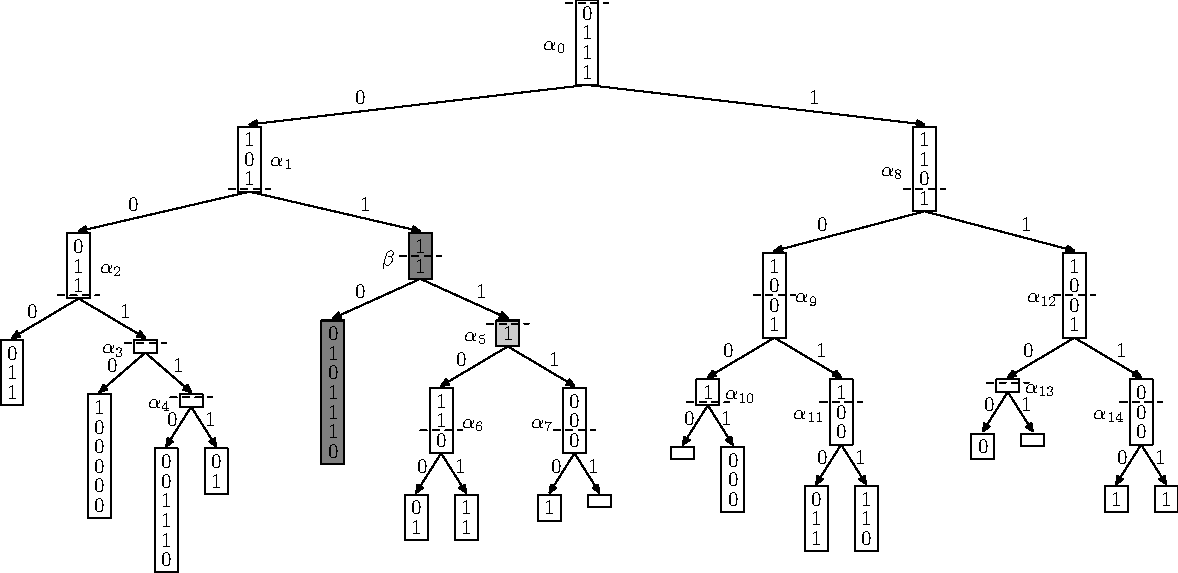
\includegraphics[scale=.6]{fig/large-example-new-1.pdf}
 \caption{\label{fig:large-example-new}The z-fast trie obtained adding $0111010111100101110$ to the trie
 of Figure~\ref{fig:large-example}: the grey nodes are those involved in the insertion. The darker ones
 are new, the lighter one is the old exit node ($\alpha_5$ in Figure~\ref{fig:large-example}, now with a different content).}
\end{figure}

Updating the compacted trie requires the usual constant number of pointer updates.
Note that if $x\preceq e_{\exit x}$ or if $\exit x$ is a leaf and $e_{\exit x}\prec x$, then $x$ 
is already present or cannot be inserted, because otherwise the set would no longer be prefix-free.

The node $\exit x$ (in Figure~\ref{fig:large-example}, it was $\alpha_{5}$) splits in two: 
a \emph{new parent node} containing only the portion
of $c_{\exit x}$ before the point at which $x$ exits (in Figure~\ref{fig:large-example-new}, this
new parent node is called $\beta$) with two children: one is a \emph{new
leaf} (the one representing $x$), and the other is the old $\exit x=\alpha_5$ but it is updated to contain only
the remaining suffix of $c_{\exit x}$.

If the exit node was a leaf, we have only one brand new internal node (the new parent node),
whose handle is to be inserted in the dictionary (the corresponding value being, of course, the new node itself).
If the exit node was internal, one of the two internal nodes involved (either the new parent, or the old node that is now a child)
has the same handle as before: so its key is already present in the dictionary; we have to change its
value only if $x$ cuts low (because in that case the handle now refers to the new parent).
The other internal node has a brand new handle, that should be inserted in the dictionary.

In the example of Figure~\ref{fig:large-example-new}, $x$ cuts high, hence the old handle ($h_{\alpha_5}=011101011111$) still
points to the same node as before. The new handle is the handle of $\beta$, that is,
$011101011$.

Deletions can be performed running backwards the insertion algorithm: to do so, one needs
the exit node, the parex , and the grandparent of the exit node. Then a single pointer
assignment to the latter node updates the trie structure: in Figure~\ref{fig:large-example},
when removing the new leaf we would set the right child pointer of $\alpha_1$ to $\alpha_5$,
and update the name of $\alpha_5$ accordingly. 

For what concerns the z-map, if the sibling of the exit node is internal and $x$ cuts low
we have to first remove the sibling, and then use it to replace the parex, as the new handle
of the sibling will be identical to the handle of the parex. Otherwise,
we just need to remove the parex.

Update bounds are trivially satisfied, as we have to update the compacted trie and at most two dictionary entries,
which can be performed within the bounds of Theorem~\ref{th:bounds} using standard techniques (note that for deletions
it is essential to recover the parex node).

\subsection{Space usage}
\label{sec:space}

From the description given in the previous sections, 
internal nodes must contain their extent and skip interval, and the dictionary must contain
handles, which might require space as much as three times that
necessary to store $S$. As long as the strings have length $O(w)$, there is asymptotically
no difference in the space usage, but in practice
while this might be acceptable for very short strings (i.e., integers),
it would be a problem for longer strings, and in particular for the signed version we will discuss in Section~\ref{sec:sign}, 
in which strings can be of length up to $2^w$.
We thus briefly describe how reduce the amount of data stored at each node, and in particular how to avoid storing additional
strings at all.

First of all, it is not necessary to store both extremes skip intervals: 
it is enough to store its left extremes, because the
right extreme of an internal node can be deduced from any of its children.

Second, we do not actually need to store handles in the dictionary: since every handle
is associated with an internal node whose extent is an extension of its handle,
the dictionary can deduce the handle from the extent and the skip interval of the internal node.

Finally, we can avoid storing the extents of internal nodes at the price of an
additional pointer per node, because the extent $e_\alpha$ of every internal
node $\alpha$ is a prefix of some string in $S$, and such strings are pointed at
in the leaves. Thus, we can just store in each internal node a reference to one
(any will do) of its descendant leaves. It is easy to make this relation between
internal nodes and leaves an injection (i.e., different nodes always point to
different leaves); by storing also in the leaf a backward reference it is
possible to perform insertions and deletions with few additional pointers assignment:
on insertion, a new leaf will be the reference leaf for the newly inserted parent node, whereas on removal\todo{???}. 
Combining these three
considerations, beyond the space necessary to
store $S$, we just need a few words per node.

\section{Signatures}
\label{sec:sign}

We now introduce the idea of replacing extents of internal nodes with fixed-length \emph{signatures}; the resulting
data structure, the simple \emph{signed} z-fast trie, can store strings of length at most $2^w$ and
perform membership queries and updates within the bounds of Theorem~\ref{th:bounds} with high probability.

\subsection{Locating exit/parex without prefix check}
\label{sec:exitorparex}

Looking back at Algorithm~\ref{algo:parex}, the reader can verify that the only string comparison
performed is the test $e_\beta\prec x$. If we remove the test, we obtain
Algorithm~\ref{algo:exitorparex}, which has a peculiar
property:

\begin{Algorithm}
\begin{algorithmic}
\STATE{\textbf{Function: } LocateExitOrParex}
\STATE{\textbf{Input:} a string $x$}
\STATE{\textbf{Output:} either $\exit x$ or $\parex x$} 
\STATE $\Sigma\leftarrow\text{empty stack}$
\STATE $a, b\leftarrow 0,|x|$
\WHILE{$a \leq b$}
        \STATE{$f\leftarrow $ the 2-fattest number in $[a\..b]$}
        \STATE{$\beta\leftarrow Z(x[0\..f))$}
        \IF{$\beta\neq\bot$} 
        	\STATE $a\leftarrow |e_\beta| + 1$ \COMMENT{Move from
        	$[a\..b]$ to 	$[|e_\beta|+1\..b]$}
        	\STATE push $\beta$ on $\Sigma$
        \ELSE
           \STATE $b\leftarrow f - 1$ \COMMENT{Move from $[a\..b]$ to
           $[a\..f - 1]$}
        \ENDIF
\ENDWHILE
\STATE{{\bf return} $\Sigma$}
\end{algorithmic}
\caption{\label{algo:exitorparex}At the end of the
execution, on the stack you will find a node $\sigma$ (on the top) and its
2-fat ancestors, where $\sigma$ is either $\exit x$ or $\parex x$.}
\end{Algorithm}


\begin{theorem}
\label{th:exitorparex}
Let $x$ be a nonempty string, and 
\[\sigma=
\begin{cases}
\parex x & \text{if $x$ cuts high or
$\exit x$ is a leaf}\\
\exit x & \text{otherwise.}
\end{cases}
\]
Let 
$\alpha_0$,~$\alpha_1$, $\dots\,$,~${\alpha}_{t}=\sigma$
be the sequence of 2-fat ancestors of $\sigma$ (in increasing handle-length order).
Let $[a\..b]$ be the interval maintained by 
  Algorithm~\ref{algo:exitorparex}. After each iteration the following
  invariant is satisfied: $a=|e_{\alpha_j}|+1$ for some $j$ and
  $|h_\sigma|\leq b$. Moreover, all values $|e_{\alpha_j}|+1$ are attained by $a$
  (in order of increasing $j$) at some point of the execution.
\end{theorem}
\begin{proof}
The proof is similar to that of Theorem~\ref{th:parex}.
Note that $h_\sigma$ is the longest handle in $Z$ that is a prefix of
$x$. 

The first value of $f$ is necessarily zero, so at the first iteration
$\beta$ is the root node, which is the first 2-fat ancestor of every node:
the root is correctly pushed onto the stack and $a=|e_{\mathrm{root}}|+1$:
if $\exit x$ is the root, we either exit immediately (because $b<a$) or in any
case the following queries all return $\bot$, and no other node is pushed onto the stack until the
end.

We now prove by induction that in the rest of execution the invariant is true.
At each step we pick the
$2$-fattest number $f\in[|e_{\alpha_i}|+1\..b]$, and change interval. Let
$\beta=Z(x[0\..f))$. We have two cases:
\begin{itemize}
  \item If $f\leq |h_\sigma|$, $x[0\..f)$
  must be the handle of a node $\beta$, as $f$ is
  2-fattest in
  $[|e_{\alpha_i}|+1\..b]\supseteq[|e_{\alpha_i}|+1\..|h_\sigma|]$.
  Moreover, necessarily $\beta=\alpha_{i+1}$ because of Lemma~\ref{lemma:twofateq}. Thus, by setting
  $a=|e_\beta|+1=|e_{\alpha_{i+1}}|+1$ the invariant is preserved.
  \item If $|h_\sigma|<f$, necessarily 
  $\beta=\bot$. Thus, by setting $b=f-1\geq|h_\sigma|$  we
    preserve the invariant.\qed
\end{itemize}
\end{proof}

Table~\ref{tab:example-query-exitorparex} shows how this algorithm behaves for the same trie
and query as in Table~\ref{tab:example-query-parex}: note that the two algorithms behave alike,
until $\beta=\alpha_5$. At that point, since Algorithm~\ref{algo:exitorparex} does not check
whether $e_\beta$ is a prefix of $x$, $\alpha_5$ is pushed onto the stack and thereafter the two executions
diverge. 

\begin{table}
\centering
%\documentclass{article}
%\usepackage{tikz}
%\usetikzlibrary{arrows, chains, fit, quotes}

%\begin{document}
	{
        \setlength\tabcolsep{0.5em}
	\begin{tabular}{|l|r|r|r|c|c|c|}
	\hline
	& $a$ & $b$ & $f$ & $\beta$ & Stack (after)\\\hline

	\rule{0pt}{2.5em}\rule[-2.5em]{0pt}{2.5em}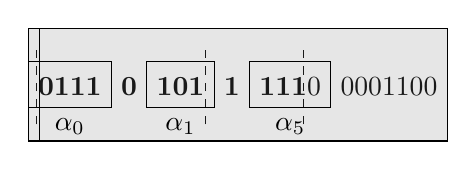
\begin{tikzpicture}[
	  baseline,
	  node distance = 0mm,
	  start chain = A going right,
	  txt/.style = {text height=2ex, text depth=0.25ex, 
	                 on chain},
	  every edge/.append style = {draw, -stealth'}
	  ]

	\node [txt] {$\mathbf{0111}$};     % nodes are in the chain
	\draw [dashed] ([xshift=3pt, yshift=-6pt]A-1.south west) -- ([xshift=3pt, yshift=6pt]A-1.north west);
	\node [txt] {$\mathbf{0}$};
	\node [txt] {$\mathbf{101}$};
	\draw [dashed] ([xshift=-3pt, yshift=-6pt]A-3.south east) -- ([xshift=-3pt, yshift=6pt]A-3.north east);
	\node [txt] {$\mathbf{1}$};
	\node [txt] {$\mathbf{111}0$};
	\draw [dashed] ([xshift=-10pt, yshift=-6pt]A-5.south east) -- ([xshift=-10pt, yshift=6pt]A-5.north east);
	\node [txt] {$0001100$};
	%
	\node (g) [draw=black, fill=black!50, fill opacity=0.2, inner ysep=12pt, inner xsep=0,
		   fit=(A-1) (A-6)] {};
	
	\node (f1)  [draw=black, inner sep=0pt, 
	             label=below:$\alpha_0$, 
	             fit=(A-1) (A-1)] {};
	\node (f3)  [draw=black, inner sep=0pt, 
	             label=below:$\alpha_1$,
	             fit=(A-3) (A-3)] {};

	\node (f5)  [draw=black, inner sep=0pt, 
	             label=below:$\alpha_5$,
	             fit=(A-5) (A-5)] {};

	\draw ([xshift=4pt, yshift=-12pt]A-1.south west) -- ([xshift=4pt, yshift=12pt]A-1.north west);
       \end{tikzpicture}
    & $0$ & $20$ & $0$ & $\alpha_0$ & $\langle \alpha_0\rangle$\\\hline

    %%%%%%
	\rule{0pt}{2.5em}\rule[-2.5em]{0pt}{2.5em}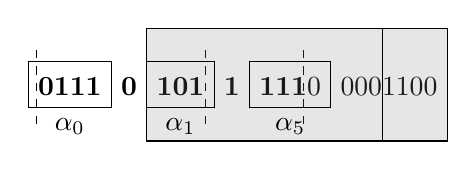
\begin{tikzpicture}[
	  baseline,
	  node distance = 0mm,
	  start chain = A going right,
	  txt/.style = {text height=2ex, text depth=0.25ex, 
	                 on chain},
	  every edge/.append style = {draw, -stealth'}
	  ]

	\node [txt] {$\mathbf{0111}$};     % nodes are in the chain
	\draw [dashed] ([xshift=3pt, yshift=-6pt]A-1.south west) -- ([xshift=3pt, yshift=6pt]A-1.north west);
	\node [txt] {$\mathbf{0}$};
	\node [txt] {$\mathbf{101}$};
	\draw [dashed] ([xshift=-3pt, yshift=-6pt]A-3.south east) -- ([xshift=-3pt, yshift=6pt]A-3.north east);
	\node [txt] {$\mathbf{1}$};
	\node [txt] {$\mathbf{111}0$};
	\draw [dashed] ([xshift=-10pt, yshift=-6pt]A-5.south east) -- ([xshift=-10pt, yshift=6pt]A-5.north east);
	\node [txt] {$0001100$};
	%
	\node (g) [draw=black, fill=black!50, fill opacity=0.2, inner ysep=12pt, inner xsep=0,
		   fit=(A-3) (A-6)] {};
	
	\node (f1)  [draw=black, inner sep=0pt, 
	             label=below:$\alpha_0$, 
	             fit=(A-1) (A-1)] {};
	\node (f3)  [draw=black, inner sep=0pt, 
	             label=below:$\alpha_1$,
	             fit=(A-3) (A-3)] {};

	\node (f5)  [draw=black, inner sep=0pt, 
	             label=below:$\alpha_5$,
	             fit=(A-5) (A-5)] {};

	\draw ([xshift=128pt, yshift=-12pt]A-1.south west) -- ([xshift=128pt, yshift=12pt]A-1.north west);
    \end{tikzpicture}
    & $5$ & $20$ & $16$ & $\bot$ & $\langle \alpha_0\rangle$\\\hline

    %%%%%%
	\rule{0pt}{2.5em}\rule[-2.5em]{0pt}{2.5em}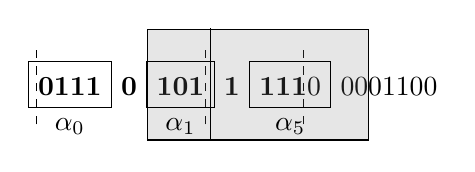
\begin{tikzpicture}[
	  baseline,
	  node distance = 0mm,
	  start chain = A going right,
	  txt/.style = {text height=2ex, text depth=0.25ex, 
	                 on chain},
	  every edge/.append style = {draw, -stealth'}
	  ]

	\node [txt] {$\mathbf{0111}$};     % nodes are in the chain
	\draw [dashed] ([xshift=3pt, yshift=-6pt]A-1.south west) -- ([xshift=3pt, yshift=6pt]A-1.north west);
	\node [txt] {$\mathbf{0}$};
	\node [txt] {$\mathbf{101}$};
	\draw [dashed] ([xshift=-3pt, yshift=-6pt]A-3.south east) -- ([xshift=-3pt, yshift=6pt]A-3.north east);
	\node [txt] {$\mathbf{1}$};
	\node [txt] {$\mathbf{111}0$};
	\draw [dashed] ([xshift=-10pt, yshift=-6pt]A-5.south east) -- ([xshift=-10pt, yshift=6pt]A-5.north east);
	\node [txt] {$0001100$};
	%
	\node (g) [draw=black, fill=black!50, fill opacity=0.2, inner ysep=12pt, inner xsep=0, minimum width=80pt, minimum height=40pt, anchor=west] at (A-3.west){};
	
	\node (f1)  [draw=black, inner sep=0pt, 
	             label=below:$\alpha_0$, 
	             fit=(A-1) (A-1)] {};
	\node (f3)  [draw=black, inner sep=0pt, 
	             label=below:$\alpha_1$,
	             fit=(A-3) (A-3)] {};

	\node (f5)  [draw=black, inner sep=0pt, 
	             label=below:$\alpha_5$,
	             fit=(A-5) (A-5)] {};

	\draw ([xshift=66pt, yshift=-12pt]A-1.south west) -- ([xshift=66pt, yshift=12pt]A-1.north west);
    \end{tikzpicture}
    & $5$ & $15$ & $8$ & $\alpha_1$ & $\langle \alpha_0, \alpha_1\rangle$\\\hline

    %%%%%%
	\rule{0pt}{2.5em}\rule[-2.5em]{0pt}{2.5em}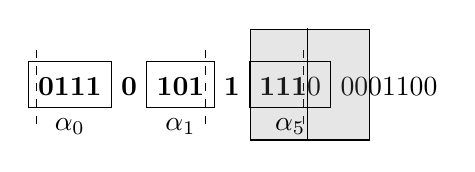
\begin{tikzpicture}[
	  baseline,
	  node distance = 0mm,
	  start chain = A going right,
	  txt/.style = {text height=2ex, text depth=0.25ex, 
	                 on chain},
	  every edge/.append style = {draw, -stealth'}
	  ]

	\node [txt] {$\mathbf{0111}$};     % nodes are in the chain
	\draw [dashed] ([xshift=3pt, yshift=-6pt]A-1.south west) -- ([xshift=3pt, yshift=6pt]A-1.north west);
	\node [txt] {$\mathbf{0}$};
	\node [txt] {$\mathbf{101}$};
	\draw [dashed] ([xshift=-3pt, yshift=-6pt]A-3.south east) -- ([xshift=-3pt, yshift=6pt]A-3.north east);
	\node [txt] {$\mathbf{1}$};
	\node [txt] {$\mathbf{111}0$};
	\draw [dashed] ([xshift=-10pt, yshift=-6pt]A-5.south east) -- ([xshift=-10pt, yshift=6pt]A-5.north east);
	\node [txt] {$0001100$};
	%
	\node (g) [draw=black, fill=black!50, fill opacity=0.2, inner ysep=12pt, inner xsep=0, minimum width=43pt, minimum height=40pt, anchor=west] at (A-5.west){};
	
	\node (f1)  [draw=black, inner sep=0pt, 
	             label=below:$\alpha_0$, 
	             fit=(A-1) (A-1)] {};
	\node (f3)  [draw=black, inner sep=0pt, 
	             label=below:$\alpha_1$,
	             fit=(A-3) (A-3)] {};

	\node (f5)  [draw=black, inner sep=0pt, 
	             label=below:$\alpha_5$,
	             fit=(A-5) (A-5)] {};

	\draw ([xshift=101pt, yshift=-12pt]A-1.south west) -- ([xshift=101pt, yshift=12pt]A-1.north west);
    \end{tikzpicture}
    & $9$ & $15$ & $12$ & $\alpha_5$ & $\langle \alpha_0, \alpha_1, \alpha_5 \rangle$\\\hline

    %%%%%%
	\rule{0pt}{2.5em}\rule[-2.5em]{0pt}{2.5em}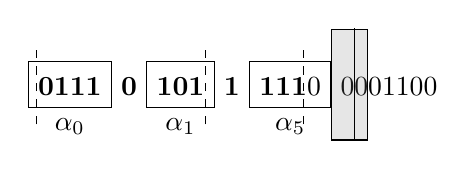
\begin{tikzpicture}[
	  baseline,
	  node distance = 0mm,
	  start chain = A going right,
	  txt/.style = {text height=2ex, text depth=0.25ex, 
	                 on chain},
	  every edge/.append style = {draw, -stealth'}
	  ]

	\node [txt] {$\mathbf{0111}$};     % nodes are in the chain
	\draw [dashed] ([xshift=3pt, yshift=-6pt]A-1.south west) -- ([xshift=3pt, yshift=6pt]A-1.north west);
	\node [txt] {$\mathbf{0}$};
	\node [txt] {$\mathbf{101}$};
	\draw [dashed] ([xshift=-3pt, yshift=-6pt]A-3.south east) -- ([xshift=-3pt, yshift=6pt]A-3.north east);
	\node [txt] {$\mathbf{1}$};
	\node [txt] {$\mathbf{111}0$};
	\draw [dashed] ([xshift=-10pt, yshift=-6pt]A-5.south east) -- ([xshift=-10pt, yshift=6pt]A-5.north east);
	\node [txt] {$0001100$};
	%
	\node (g) [draw=black, fill=black!50, fill opacity=0.2, inner ysep=12pt, inner xsep=0, minimum width=13pt, minimum height=40pt, anchor=west] at (A-5.east){};
	
	\node (f1)  [draw=black, inner sep=0pt, 
	             label=below:$\alpha_0$, 
	             fit=(A-1) (A-1)] {};
	\node (f3)  [draw=black, inner sep=0pt, 
	             label=below:$\alpha_1$,
	             fit=(A-3) (A-3)] {};

	\node (f5)  [draw=black, inner sep=0pt, 
	             label=below:$\alpha_5$,
	             fit=(A-5) (A-5)] {};

	\draw ([xshift=118pt, yshift=-12pt]A-1.south west) -- ([xshift=118pt, yshift=12pt]A-1.north west);
    \end{tikzpicture}
    & $14$ & $15$ & $14$ & $\bot$ & $\langle \alpha_0, \alpha_1, \alpha_5\rangle$\\\hline

    %%%%%%
	\rule{0pt}{2.5em}\rule[-2.5em]{0pt}{2.5em}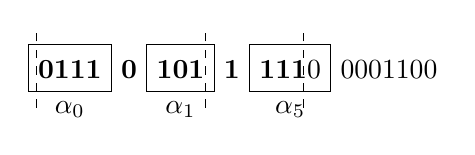
\begin{tikzpicture}[
	  baseline,
	  node distance = 0mm,
	  start chain = A going right,
	  txt/.style = {text height=2ex, text depth=0.25ex, 
	                 on chain},
	  every edge/.append style = {draw, -stealth'}
	  ]

	\node [txt] {$\mathbf{0111}$};     % nodes are in the chain
	\draw [dashed] ([xshift=3pt, yshift=-6pt]A-1.south west) -- ([xshift=3pt, yshift=6pt]A-1.north west);
	\node [txt] {$\mathbf{0}$};
	\node [txt] {$\mathbf{101}$};
	\draw [dashed] ([xshift=-3pt, yshift=-6pt]A-3.south east) -- ([xshift=-3pt, yshift=6pt]A-3.north east);
	\node [txt] {$\mathbf{1}$};
	\node [txt] {$\mathbf{111}0$};
	\draw [dashed] ([xshift=-10pt, yshift=-6pt]A-5.south east) -- ([xshift=-10pt, yshift=6pt]A-5.north east);
	\node [txt] {$0001100$};
	%
	
	\node (f1)  [draw=black, inner sep=0pt, 
	             label=below:$\alpha_0$, 
	             fit=(A-1) (A-1)] {};
	\node (f3)  [draw=black, inner sep=0pt, 
	             label=below:$\alpha_1$,
	             fit=(A-3) (A-3)] {};

	\node (f5)  [draw=black, inner sep=0pt, 
	             label=below:$\alpha_5$,
	             fit=(A-5) (A-5)] {};

    \end{tikzpicture}
    & $14$ & $13$ & - & - & $\langle \alpha_0, \alpha_1, \alpha_5\rangle$\\\hline
    \end{tabular}
    }


%\end{document}

\vspace*{.5cm}
\caption{\label{tab:example-query-exitorparex}Execution of Algorithm~\ref{algo:exitorparex} on the trie of Figure~\ref{fig:large-example}
with the same input as in Table~\ref{tab:example-query-parex}: note how the two algorithms start
alike, but diverge after hitting the exit node $\alpha_5$.}
\end{table}

A few remarks are in order:
\begin{itemize}
  \item Algorithm~\ref{algo:exitorparex} completes in at most $\lg|x|$ iterations, like
  Algorithm~\ref{algo:parex}, but requires no string comparison.  
    \item As in the case of Algorithm~\ref{algo:parex}, at the end of Algorithm~\ref{algo:exitorparex} the returned stack contains
  all and only the 2-fat ancestors of $\sigma$ in increasing handle-length order (the empty
  stack if $\sigma=\bot$).
  \item Given the output of Algorithm~\ref{algo:exitorparex}, it is possible to 
  obtain the exit node as follows: if the output is the empty stack, $\exit x$ is the root;
  otherwise the exit node can be obtained by the LocateExit function described in Algorithm~\ref{algo:exit}.
  The function first checks if the node is the parex or the exit node, and in the former case uses
  one bit of $x$ to access the correct child.
\end{itemize}

\begin{Algorithm}
\begin{algorithmic}
\STATE{\textbf{Function: } LocateExit}
\STATE{\textbf{Input:} a string $x$ and the node $\sigma$ on the top of the stack produced by Algorithm~\ref{algo:exitorparex}.}
\STATE{\textbf{Output:} $\exit x$} 
\IF{$\sigma=\bot$}
	\STATE{{\bf return} the root}
\ENDIF
\IF{$e_\sigma\prec x$}
	\IF{$x[|e_\sigma|]=0$}
		\STATE{{\bf return} the left child of $\eta$}
	\ELSE
		\STATE{{\bf return} the right child of $\eta$}
	\ENDIF
\ELSE
	\STATE{{\bf return} $\eta$}
\ENDIF
\end{algorithmic}
\caption{\label{algo:exit}This function locates the exit node of $x$, given the output of Algorithm~\ref{algo:exitorparex}.}
\end{Algorithm}




\subsection{A z-map with false positives}

Algorithm~\ref{algo:exitorparex} at this point may not seem to be particularly useful: its
only application is an alternative way (if only slightly faster, in practice) to find the exit node of a
string when answering membership queries.

However, we will be interested in what happens when $Z$ may nondeterministically
return \emph{false positives}: by this we mean that $Z$ will always return a
correct internal node on keys that are part of its domain (i.e., the handles of
the internal nodes), but it may nondeterministically return an internal node
even for a key that is not a handle.

\begin{theorem}
\label{th:errors}
Assume that during the execution of Algorithm~\ref{algo:exitorparex} on the string $x$ the
function $Z$ may nondeterministically return false positives.
Then, letting $0=\;$\lst fk be consecutive values of $f$ for which
$Z\bigl(x[0\..f_i)\bigr)=\beta_i\neq\bot$, if $\beta_k$ 
is not a false positive then this is also true for each $\beta_i$, $0\leq i<k$.
\end{theorem}
\begin{proof}
We assume without loss of generality that the length of the handle of a false positive
is equal to the length of the key.\footnote{If you have a $Z'$ that may sometimes return false positives $\beta$ with
$|h_\beta|\neq f$, just define a new $Z$ that behaves exactly like $Z'$, but in those cases returns $\bot$, instead.} 

Note that $f_0<f_1<\cdots<f_k$ (by the way we change the value of $a$ when $Z$ does not return $\bot$
and by our assumption $|e_\beta|\geq |h_\beta|=f$).
If the $k$-th call to $Z$ was not a false positive we have
\[
x[0\..f_i) \preceq x[0\..f_k) = x\bigl[0\..|h_{\beta_k}|\bigr) =
h_{\beta_k}\preceq x,
\]
so $f_i\leq f_k=|h_{\beta_k}|\leq|h_\sigma|$ (because of the very definition of
$\sigma$ in the statement of Theorem~\ref{th:exitorparex}, as the node with the longest
handle that is a prefix of $x$). Thus, the second case ($f>|h_\sigma|$) in
the proof of Theorem~\ref{th:exitorparex} never occurred in the steps preceding the $k$-th, 
and each $x[0\..f_i)$ is a handle, so each $\beta_i$ is a true positive.\qed
\end{proof}

In other words, after the first false positive is obtained, the following calls will always yield
either $\bot$ or a false positive. Hence, if the final non-$\bot$ call is not a false positive, then
no false positives were ever returned during the execution of the algorithm.


\subsection{Implementing the z-map}
\label{sec:dict}


Theorem~\ref{th:errors} has an implication that we will use for implementing
the signed z-fast trie: we can run Algorithm~\ref{algo:exitorparex} with a z-map
returning false positives and check that the result is correct at the end.
The advantage of this approach is that we can implement the z-map as a suitable dictionary
on \emph{signatures} of handles, rather than on the handles themselves. At that point,
if the signatures are sufficiently short, accessing the map requires constant time (except for the computation of the signature).


\paragraph{Handling errors.}
The only important property we must preserve, which is necessary for Theorem~\ref{th:errors} to work, 
 is that the dictionary must always return
the correct answer on the signature of an existing handle. For the moment, let us assume that
there are no duplicate signatures (i.e., that all handles have distinct signatures).

Signatures of handles are computed at construction/insertion time,
whereas signatures for prefixes of the query string $x$ can be computed incrementally: after a
preprocessing using time $O(|x|/w)$ and $O(|x|/B)$ I/Os, computing a signature
for an arbitrary prefix of $x$ takes constant time.

Assuming we have signatures of length $c\lg n + \lg w$, 
it is easy to see that the probability of performing $w$ probes (we will do at most
$w$ probes on input $|x|$, because $\lg |x| \leq \lg 2^w=w$)
without getting a false positive is at least $1-1/n^{c-1}$: 
indeed,  the probability that a given prefix induces a false positive 
is at most $n/(wn^c)$ (by a union bound), so hitting a false positive during a query
(i.e., any of the at most $w$ tests) 
of a false positive is at most $1/n^{c-1}$.

Thus,
Algorithm~\ref{algo:exitorparex} will end with the correct output in time $O(|x|/w +\lg|x|)$ with
high probability, because of Theorem~\ref{th:errors}. Note that since $n$ is not known in advance, the signatures
must actually be $cw+\lg w=O(w)$ bits long (we assume, as usual, that the set
size is at most $2^w$, so $c\lg n\leq cw$).

At the end of the algorithm, we just need to check if $h_\beta\preceq x$
to see if the result is correct (which we can do in time $O(|x|/w)$). 
Otherwise, we re-run the algorithm using actual keys
instead of signatures if something went wrong (this requires time
$O((|x|/w+1)\lg|x|)$ and $O((|x|/B+1)\lg|x|)$ I/Os). 

\paragraph{Duplicate signatures.} 
Duplicate signatures require some attention: if two existing handles have the same signatures, we must somehow
record that whenever \emph{that} signature is queried for, the actual prefix must be compared in order to determine
which node should be returned. 
This means that if during the execution of Algorithm~\ref{algo:exitorparex} we try to query the map with an
existing but duplicate signature, an explicit comparison will be needed. With the same analysis as above, 
we obtain that the probability of hitting a duplicate signature during the execution of the
algorithm is at most $1/n^{c-1}$. So the probability that we have to re-run the algorithm using 
the actual keys because of duplicate signatures is at most $1/n^{c-1}$.

\smallskip
Summarizing the two cases above, with probability at least $1-2/n^{c-1}$ there will be no need to run the algorithm on actual keys,
because neither false positive nor duplicate keys will be met. 


\section{Jump pointers}
\label{sec:jumppointers}

We are now going to complete the description of the z-fast trie by adding  
two additional pointers per node. On the leaves, such pointers are used to 
keep the keys in a doubly linked list (i.e., pointers pointing to the next/previous leaf in lexicographic
order). The additional pointers of an internal node $\alpha$ will be
denoted by $J_\alpha^-$ and $J_\alpha^+$ and will be called \emph{jump pointers}.
Their role is making it possible to reach quickly the leftmost and rightmost descendant
leaves of $\alpha$, respectively.\footnote{We recall that a \emph{right (left) descendant} is either the right (left) child,
or a right (left) descendant of the right (left) child.}
 
The \emph{left} jump pointer $J_\alpha^-$ of a node
$\alpha$ points somewhere along the path defined recursively by the left child
pointers (analogously for the \emph{right} jump pointer $J_\alpha^+$). How far the
pointer goes depends on some arithmetics related to 2-fattest numbers. Our goal
is to position jump pointers so that if the rightmost (largest) leaf under node
$\alpha$ contains the string $x$, in $O(\lg|x|)$ steps we can get to that leaf. At
the same time, when we perform insertions or deletions we want to be
able to update the pointers in time $O(\lg|e_{\exit x}|)$, where $x$ is the
string added to/removed from the trie.
We start with a definition.

\begin{definition}
An internal node $\alpha$ \emph{intercepts} $k\in \mathbf N\cup\sing\infty$ if $k$ belongs to the
skip interval of $\alpha$; a leaf $\alpha$ intercepts $k\in \mathbf N\cup\sing\infty$ if $k\geq i_\alpha$, that
is, if $k$ belongs to the skip interval of $\alpha$ or is larger than its right
extreme. Given an internal node $\alpha$, its \emph{left (right) jump pointer}
points to its unique left (right) descendant that intercepts $|h_\alpha|'$.
\end{definition}

The intuition behind this definition is that jump pointers point near for nodes
with lean handles, and point far for nodes with fat handles. Of course,
since when we follow a jump pointer of $\alpha$ we land into a node $\beta$
whose skip interval contains $|h_\alpha|'$, the handle of node
$\beta$ will have strictly fatter length than $|h_\alpha|$: as a consequence, 
we never need more than $\lg|x|$ jumps to reach the leaf containing the string
$x$. Note that, in particular, the left and right jump pointers of the root 
point to the first and last element in $S$.
Figure~\ref{fig:bigtrie} shows a graphical display of a sample z-fast trie
endowed with jump pointers.

% 
 \begin{figure}
 \begin{center}
 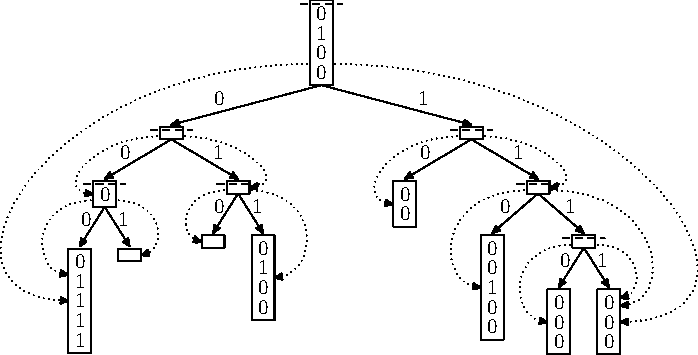
\includegraphics[scale=.9]{fig/small-example-1.pdf}
 \caption{\label{fig:bigtrie}A z-fast trie with dotted lines representing jump
 pointers. Dashed lines represent handles.}
 \end{center}
 \end{figure}

Following left (right, respectively) jump pointers from a node $\beta$ we eventually reach the left-descendant 
(right-descendant, respectively) leaf, hereafter just called \emph{leftmost leaf under $\beta$} (rightmost leaf, respectively).
These two nodes are essential for the computation of predecessor/successor, prefix, and range queries: 
\begin{lemma}
\label{lemma:descleaves}
If $x$ exits on the left, then it is smaller than or equal to the leftmost leaf under $\exit x$ and
larger than every leaf preceding it.
If $x$ exits on the right, then it is larger than the rightmost leaf of $\exit x$
and smaller than every leaf following it.
\end{lemma}
\begin{proof}
If $x$ exits on the left, then either $x \preceq e_{\exit x}$ or $x$ and $e_x$ are $\preceq$-incomparable and the 
bit of $x$ after the longest common prefix is a $0$: in both cases, $x$ is smaller than every leaf under $\exit x$. 
Moreover, $x$ is larger than the previous leaves because of the definition of exit node.

If $x$ exits on the right, then $x$ and $e_x$ are $\preceq$-incomparable and the 
bit of $x$ after the longest common prefix is a $1$: in this case, $x$ is larger than every leaf
under $\exit x$. 
Again, $x$ is smaller than the following leaves because of the definition of exit node. \qed
\end{proof}
\todo[inline]{Check that the statement is correct}



\section{Queries}

We now proceed to describe how the various types of queries discussed in 
Theorem~\ref{th:bounds} and~\ref{th:boundslong} are handled by the z-fast trie,
and prove the associated time bounds. In this presentation we shall refer to the
case of long strings and signature-based tries (the case of short strings is similar, and simpler);
all time bounds hold only with high probability (whereas the corresponding bounds for short strings are worst-case bounds).
All algorithms will need to locate one (or two) exit nodes, and they will do so using Algorithm~\ref{algo:exitorparex}
followed by a check of correctness (Theorem~\ref{th:errors}): if the correctness check fails (which happens
with negligible probability), the algorithm resorts to exact search; otherwhise, it will proceed
locating the exit node through Algorithm~\ref{algo:exit}.  

In all cases, the I/O bounds are easily proved as we scan $x$ (or $y$)
a fixed number of times to preprocess them so to obtain hashes of prefixes in
constant time, or to compare them to other strings.

\subsection{Predecessor/successor queries} 
\label{sec:predsucc}

In time $O(|x|/w + \lg|x|)$ we recover the
exit node of $x$ using Algorithm~\ref{algo:exit} (preceded by error detection and correction, as needed). 
Then, by examining $e_{\exit
x}$ and $x$ we decide in time $O(|x|/w)$ whether $x$ exits on the left or on the
right. By moving through jump pointers to the
leftmost (rightmost, respectively) leaf, we can find the successor (predecessor, resp.) of $x$
in time $O(\lg\max\{\?|x^-|,|x^+|\?\})$;
then, possibly after a single access to the doubly linked list of leaves, we can return
the result, using Lemma~\ref{lemma:descleaves}. For example, if and we want to obtain the
predecessor $x^-$ of $x$, and $x$ exits on the right, we just return the rightmost leaf under $\exit x$; 
if $x$ exits on the left, we return the \emph{predecessor} of the leftmost leaf under $\exit x$, instead. 
The Algorithm is presented in~\ref{algo:predsucc}.

\begin{Algorithm}
\begin{algorithmic}
\STATE{\textbf{Function: } Predecessor/Successor}
\STATE{\textbf{Input:} a string $x$}
\STATE{\textbf{Output:} $x^-$ and $x^+$, the predecessor and successor of $x$ in $S$} 
\STATE{$\Sigma\leftarrow\text{LocateExitOrParex}(x)$}
\IF{$\Sigma=\emptyset$}
	\STATE{$\eta\leftarrow\text{root}$}
\ELSE
	\STATE{$\eta\leftarrow\text{LocateExit}(\text{top}(\Sigma))$}
\ENDIF
\IF{$x$ exits on the left}
	\STATE{$\lambda\leftarrow\text{prev$(\text{leftmost leaf under $\eta$})$}$}
	\STATE{$\rho\leftarrow\text{leftmost leaf under $\eta$}$}
\ELSE
	\STATE{$\lambda\leftarrow\text{rightmost leaf under $\eta$}$}
	\STATE{$\rho\leftarrow\text{next$(\text{rightmost leaf under $\eta$})$}$}
\ENDIF
\STATE{{\bf return } $e_{\lambda}, e_{\rho}$}
\end{algorithmic}
\caption{\label{algo:predsucc}Predecessor and successor queries.}
\end{Algorithm}


\subsection{Prefix queries}  

In time $O(|x|/w + \lg|x|)$ we recover the
exit node of $x$ using Algorithm~\ref{algo:exit}. We then check in time
$O(|x|/w)$ that $x\preceq e_{\exit x}$: if so, we use the left jump pointers to
reach the leftmost and rightmost leaves under $\exit x$, and then we
enumerate the leaves in the subtree using the pointers of the linked list of leaves, starting from the
leftmost leaf and stopping at the rightmost one (the enumeration requires
$O(k)$ time to output $k$ elements). If $x\not\preceq e_{\exit x}$ the output is
empty. Note that the test $x\preceq e_{\exit x}$ is sufficient to answer
existential queries. 

\subsection{Range queries} 

\paragraph{Existential range queries.}
For the existential range query $[x\..y)$ (``Does there exist an $s \in S$ such that $x \leq s<y$?'') we first locate $\exit
x$ and $\exit y$ using Algorithm~\ref{algo:exit} in time
$O(\max\{\?|x|,|y|\?\}/w + \lg\max\{\?|x|,|y|\?\})$. Starting from $\exit x$
we follow left or right jump pointers (depending on whether $x$ exits on the left or right) until
reaching a node $\alpha$ such that $\alpha$  is 
a leaf or $|e_\alpha|\geq|y|$.
Similarly, starting from $\exit y$ we follow left or right jump pointers (depending on whether $y$ exits on the left or right) until
reaching a node $\beta$ such that either $\beta$ is 
a leaf, or $|e_\beta|\geq|x|$. These searches take time $O(\lg\max\{\?|x|,|y|\?\})$.

We have the following cases:
\begin{itemize}
  \item if $x$ exits on the left, the answer is ``true'' if and only if $e_\alpha<y$, because all keys
  greater than or equal $x$ are also necessarily greater than or equal to $e_\alpha$, 
  and all keys starting with $e_\alpha$ are necessarily smaller than $y$ (because is $\alpha$ is a leaf or $|e_\alpha|\geq |y|$).
  \item similarly, if $y$ exits on the right, the answer is ``true'' if and only if $x \leq e_\beta$;
  \item in the remaining case (i.e., if $x$ exits on the right and $y$ exits on the left), the answer is ``true'' if the leaf
  following $x^-$ is not $y^+$, because the leaf following $x^-$ is the first key greater than or equal to $x$, and $y^+$ is the 
first key greater than or equal o $y$.
\end{itemize}

We now relieve the third case from its dependence on
$|x^-|$ and $|y^+|$ (which are unbounded in $|x|$ and $|y|$). 
Note that if $x$ exits on the right
and $y$ exits on the left then $\lcp(x,y)$ (the longest common prefix of $x$ and $y$) is necessarily the extent of some node $\eta$:
in fact $x$ and $y$ cannot exit earlier than $\lcp(x,y)$ (or otherwise they would exit in the same 
direction) and conversely they go to different children after $\lcp(x,y)$.

We can recover this node $\eta$ using Algorithm~\ref{algo:exitorparex} in time
$O(\max\{\?|x|,|y|\?\}/w + \lg\max\{\?|x|,|y|\?\})$. The left (right, respectively) child of $\eta$
brings to the exit node of $x$ ($y$, respectively). We then follow the right
(left, respectively) jump pointers of the left (right, respectively) child of
$\eta$ until
reaching a node $\alpha$ ($\beta$, respectively) such that $|e_\alpha|\geq|x|$
($|e_\beta|\geq|y|$, respectively). This requires time $O(\lg|x|)$
($O(\lg|y|)$, respectively). The output is not empty iff $x\leq e_\alpha$
or $e_\beta< y$.
The resulting algorithm is presented in Algorithm~\ref{algo:range}.

\begin{Algorithm}[htbp]
\begin{algorithmic}
\STATE{\textbf{Function: } IsNonempty}
\STATE{\textbf{Input:} $x$ and $y$, with $x<y$}
\STATE{\textbf{Output:} whether $S\cap [x\..y)=\emptyset$} 
\STATE{$\alpha\leftarrow\text{LocateExit($x$)}$}
\IF{$x$ exits on the left}
	\WHILE{$\alpha$ is not a leaf \AND $|e_\alpha|<|y|$}
		\STATE{$\alpha\leftarrow J_\alpha^-$}
	\ENDWHILE
	\STATE{{\bf return} $e_\alpha<y$}

\ENDIF
\STATE{$\beta\leftarrow\text{LocateExit($y$)}$}
\IF{$y$ exits on the right}
	\WHILE{$\beta$ is not a leaf \AND $|e_\beta|<|x|$}
		\STATE{$\beta\leftarrow J_\beta^+$}
	\ENDWHILE
	\STATE{{\bf return} $x \leq e_\beta$}
\ENDIF
	\STATE{$\eta\leftarrow\text{LocateExit$(\lcp(x,y))$}$} \COMMENT{Use Algorithm~\ref{algo:exitorparex} followed by Algorithm~\ref{algo:exit}}
	\STATE{$\alpha\leftarrow\text{the left child of $\eta$}$}
	\WHILE{$\alpha$ is not a leaf \AND $|e_\alpha|<|x|$}
		\STATE{$\alpha\leftarrow J_\alpha^+$}
	\ENDWHILE
	\IF{$x\leq e_\alpha$}
	\STATE {{\bf return} true}
	\ENDIF
	\STATE{$\beta\leftarrow\text{the right child of $\eta$}$}
	\WHILE{$\beta$ is not a leaf \AND $|e_\beta|<|y|$}
		\STATE{$\beta\leftarrow J_\beta^-$}
	\ENDWHILE
	\STATE{{\bf return} $e_\beta<y$}
\end{algorithmic}
\caption{\label{algo:range}Existential range queries.}
\end{Algorithm}


\paragraph{Enumerative range queries.} Standard (i.e., enumerative) range queries can be answered easily 
noting that after the range emptiness check either we know $x^-$ ($y^+$, respectively), or we can recover it
in time $O(k)$, where $k$ is the size of the output. For example, if $x$
exits on the left and the output is not empty then the entire subtree under $\exit x$ is part of the output, and thus
it has size and depth bounded by $k$: we conclude that following left jump pointers
up to $x^+$ has cost $O(k)$ (recovering $x^-$ is then trivial).
 

\section{Additional updates}

In this section we will discuss how to update the additional pointers (jump pointers and list pointers) after the insertion or deletion of a string. 

We remark that to insert a new leaf into the doubly linked list of leaves, if
$x$ exits on the right (left, respectively) we must insert the new leaf
immediately before $x^+$ (immediately after $x^-$, respectively):
section~\ref{sec:predsucc} discussed how to locate predecessors and successors.



\paragraph{Jump pointers of the new node.}
The new parent node $\beta$ (see Figure~\ref{fig:large-example-new}) will
need to have its jump pointers set; one of them will simply point to the new leaf, whereas
to set the other we need to look for the left/right descendant intercepting $|h_\beta|'$.
Since $|h_\beta|'-|h_\beta|\leq |h_\beta|\leq |x|$, we can start our search from the left/right
child of $\beta$ and follow at most $\lg |x|$ jump pointers to find the intercepting node.
The fact that we can simply follow jump pointers can be proven as follows: suppose by contradiction that
following the jump pointers we reach some node $\eta$ (a left/right descendant of $\beta$) that does not yet intercept
$|h_\beta|'$ but is such that one of its proper left (right) descendants
$\gamma$ intercepts $|h_\beta|'$. If $\gamma$ was not a descendant of the left/right jump of $\eta$, then
\[
	|h_\eta| < i_\gamma \leq |h_\beta|'\leq j_\gamma  < |h_\eta|',
\]
but $|h_\beta|_\prime<|h_\eta|$, so $|h_\beta|_\prime<|h_\eta|<|h_\beta|'$: by the parenthesis property (Lemma~\ref{lemma:paren}),
we conclude that $|h_\eta|'\leq |h_\beta|'$, a contradiction. 

\paragraph{Updating jump pointers.}
Let us now consider how the jump pointers of existing nodes should be updated.
A node $\alpha$ \emph{crosses} a node
$\beta$ if $e_\alpha\preceq e_\beta$ (i.e., $\alpha$ is an ancestor of $\beta$) 
and $|h_\alpha|'\geq i_\beta$ (i.e., $\alpha$
potentially jumps to some left or right descendant of $\beta$). When inserting a
new string with exit node $\beta$, only nodes crossing $\beta$ might need to change their
jump pointers. The fundamental combinatorial fact that we will use to update
quickly the z-fast trie is the following connection between fat binary search
and jump pointers:
\begin{theorem}
\label{th:fatanc}
The nodes crossing $\beta$ are a subset of the 2-fat ancestors of its parent
$\gamma$.
\end{theorem}
\begin{proof}
Let $\xi$ be an ancestor of  $\gamma$ that is not a 2-fat ancestor, that is,
$|h_\gamma|_{(k+1)}<|h_\xi|<|h_\gamma|_{(k)}$ for some $k\geq 0$. Then, by Lemma~\ref{lemma:semipar}
we have $|h_\xi|'\leq|h_\gamma|_{(k)}\leq |h_\gamma|<i_\beta$.
 \end{proof}

Figure~\ref{fig:jumpline} shows pictorially Theorem~\ref{th:fatanc}. Note that not all the jump pointers of 2-fat ancestors need to be updated: actually, we
need to update only pointers to some nodes that are left (right) descendant of
$\beta$. 

 \begin{figure}[htbp]
 \centering
 		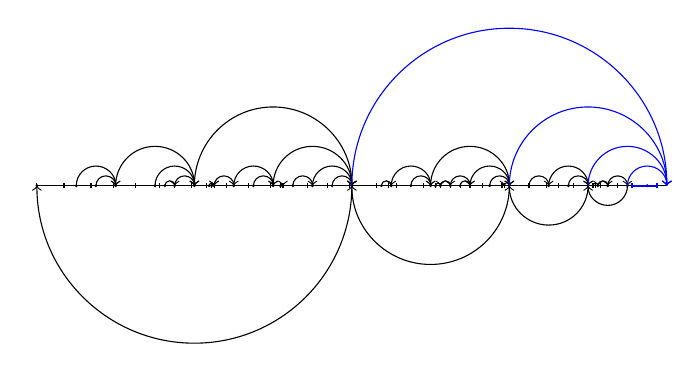
\begin{tikzpicture}


				% Main line
				\draw (0, 0) -- (8, 0);
				% Ticks (skip intervals extreme)
				\foreach \x in {0.0,0.34375,0.6875,0.96875,1.25,1.5625,1.75,1.96875,2.15625,2.21875,2.25,2.40625,2.6875,2.96875,3.09375,3.125,3.4375,3.6875,3.96875,4.3125,4.46875,4.5625,4.90625,5.0625,5.125,5.25,5.375,5.5,5.65625,5.90625,5.9375,6.25,6.46875,6.625,6.8125,7.0625,7.09375,7.15625,7.375,7.5625,7.875}
					\draw (\x, -0.03) -- (\x, 0.03) node[below]{};
				% Skip interval of beta
				\draw [thick, color=blue] (7.5625, 0) -- (7.875, 0);
				\draw [thick, color=blue] (7.5625, -0.03) -- (7.5625, 0.03) node[below]{};
				\draw [thick, color=blue] (7.875, -0.03) -- (7.875, 0.03) node[below]{};
				% Handles
				\foreach \x in {0.0,0.5,0.75,1.0,1.5,1.625,1.75,2.0,2.1875,2.21875,2.25,2.5,2.75,3.0,3.09375,3.25,3.5,3.75,4.0,4.375,4.5,4.75,5.0,5.0625,5.125,5.25,5.375,5.5,5.75,5.90625,6.0,6.25,6.5,6.75,7.0,7.0625,7.125,7.25,7.5,7.75}
					\filldraw (\x, 0) circle (0.01);
				\filldraw [color=blue] (7.75, 0) circle (0.01);
				% Backjumps
				\draw[->](7.5, 0) arc (0:-180:0.25);
				\draw[->](7.0, 0) arc (0:-180:0.5);
				\draw[->](6.0, 0) arc (0:-180:1.0);
				\draw[->](4.0, 0) arc (0:-180:2.0);
				% Jumps
				\draw[->](0.5, 0) arc (180:0:0.25);
				\draw[->](0.75, 0) arc (180:0:0.125);
				\draw[->](1.0, 0) arc (180:0:0.5);
				\draw[->](1.5, 0) arc (180:0:0.25);
				\draw[->](1.625, 0) arc (180:0:0.0625);
				\draw[->](1.75, 0) arc (180:0:0.125);
				\draw[->](2.0, 0) arc (180:0:1.0);
				\draw[->](2.1875, 0) arc (180:0:0.03125);
				\draw[->](2.21875, 0) arc (180:0:0.015625);
				\draw[->](2.25, 0) arc (180:0:0.125);
				\draw[->](2.5, 0) arc (180:0:0.25);
				\draw[->](2.75, 0) arc (180:0:0.125);
				\draw[->](3.0, 0) arc (180:0:0.5);
				\draw[->](3.09375, 0) arc (180:0:0.015625);
				\draw[->](3.25, 0) arc (180:0:0.125);
				\draw[->](3.5, 0) arc (180:0:0.25);
				\draw[->](3.75, 0) arc (180:0:0.125);
				\draw[->][color=blue](4.0, 0) arc (180:0:2.0);
				\draw[->](4.375, 0) arc (180:0:0.0625);
				\draw[->](4.5, 0) arc (180:0:0.25);
				\draw[->](4.75, 0) arc (180:0:0.125);
				\draw[->](5.0, 0) arc (180:0:0.5);
				\draw[->](5.0625, 0) arc (180:0:0.03125);
				\draw[->](5.125, 0) arc (180:0:0.0625);
				\draw[->](5.25, 0) arc (180:0:0.125);
				\draw[->](5.375, 0) arc (180:0:0.0625);
				\draw[->](5.5, 0) arc (180:0:0.25);
				\draw[->](5.75, 0) arc (180:0:0.125);
				\draw[->](5.90625, 0) arc (180:0:0.015625);
				\draw[->][color=blue](6.0, 0) arc (180:0:1.0);
				\draw[->](6.25, 0) arc (180:0:0.125);
				\draw[->](6.5, 0) arc (180:0:0.25);
				\draw[->](6.75, 0) arc (180:0:0.125);
				\draw[->][color=blue](7.0, 0) arc (180:0:0.5);
				\draw[->](7.0625, 0) arc (180:0:0.03125);
				\draw[->](7.125, 0) arc (180:0:0.0625);
				\draw[->](7.25, 0) arc (180:0:0.125);
				\draw[->][color=blue](7.5, 0) arc (180:0:0.25);


		\end{tikzpicture}


 \caption{\label{fig:jumpline}Theorem~\ref{th:fatanc}: the blue segment represents the skip interval of the exit node $\beta$, preceded by the
 skip intervals of its parent $\gamma$ and its ancestors. Every skip interval contains a small dot representing the length of its handle. The arcs
 below are the backjumps of $|h_\gamma|$, pointing to its 2-fat ancestors. The arcs above are the jumps of $|h_\xi|$ for every ancestor $\xi$; in blue are
 the ones that cross $\beta$. As the reader can see, the blue arcs all arise from 2-fat ancestors.}
 \end{figure}
 
 
To understand better which of the 2-fat ancestors of the parex should actually be updated, and how, we 
first observe that what happens depends basically on two conditions: whether the inserted string $x$ exits on
the right or on the left, and whether the exit node is a left or a right child.
We will only discuss the case in which the exit node is a left child (the other one being absolutely symmetrical).
Figure~\ref{fig:jumpadjustment} shows an example of this situation: (a) is the original trie, with the
exit node highlighted (in grey). Some of the 2-fat ancestors of its parent have left jumps pointing either directly
to the exit node or to some of its left descendants, and those jump pointers may need to be updated; note that the first time that in the ancestry line 
we meet a right child (in the Figure, when the zigzag line of ancestors turns to the left) we start finding jumps that
will point to some node to the left of the whole subtree rooted at the exit node: those jumps do not
need any update. 

What will happen to the pointers that may require an update depends on whether the new string $x$ exits on the left or on the right. 
In (b) we show the trie after the insertion when $x$ exits on the left. In dark grey the reader 
can see the new leaf
and the new internal node (that represents the upper part of the exit node), whereas in lighter grey 
we represent what remains of the exit node.
The new leftmost path now only contains the two dark grey nodes, and all the left jump pointers will have to
be conveyed to one of them (depending on whether they used to land in the upper part of the exit node or not).

In (c) we show the trie after the insertion when $x$ exits on the right. 
The new leftmost path now contains the same nodes as before, plus the new internal (dark grey) node.
The only left jump pointers that need to be updated are those that used to land in the upper part of the exit node.
    
  
\begin{figure}[htbp]
 \centering
 \begin{tabular}{ccc}
 		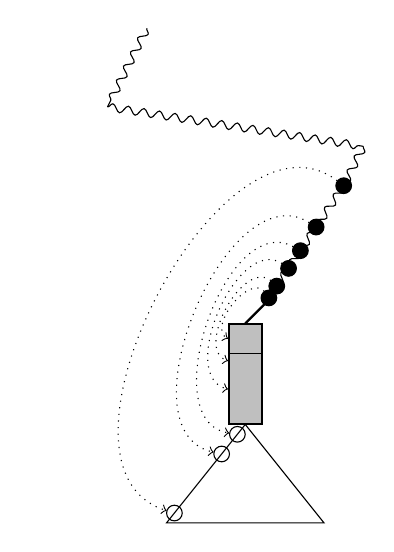
\begin{tikzpicture}[scale=0.25,every node/.style={scale=0.6}]
				\draw[decoration={snake, amplitude=0.5mm, segment length=2mm}] decorate{(0, 19) -- (-2, 15)};
				\draw[decoration={snake, amplitude=0.5mm, segment length=2mm}] decorate{(-2, 15) -- (11, 13)};
				\draw[decoration={snake, amplitude=0.5mm, segment length=2mm}] decorate{(11, 13) -- (10, 11)};
				\draw[decoration={snake, amplitude=0.5mm, segment length=2mm}] decorate{(10, 11) -- (6, 5)                     % last (right-directed) {snake, amplitude=0.5mm, segment length=2mm}
					node[pos=0, draw, circle, fill, radius=0.1pt] (sa) {}           % starting points of jump pointers
					node[pos=0.35, draw, circle, fill, radius=0.1pt] (sb) {} 
					node[pos=0.55, draw, circle, fill, radius=0.1pt] (sc) {} 
					node[pos=.7, draw, circle, fill, radius=0.1pt] (sd) {} 
					node[pos=.85, draw, circle, fill, radius=0.1pt] (se) {} 
					node[pos=.95, draw, circle, fill, radius=0.1pt] (sf) {} 
				};
				% last arc, exit node
				\draw[thick] (6,5) -- (5, 4)
					node (exit) [draw, rectangle, fill=lgray, minimum width=20, minimum height=60, anchor=north] {}; 
				% exit node division
				\coordinate (dividinglineleft) at ($(exit.north west)!0.3!(exit.south west)$);
				\coordinate (dividinglineright) at ($(exit.north east)!0.3!(exit.south east)$);
				\draw (dividinglineleft) -- (dividinglineright);
				% ending points within node
				\coordinate (ef) at ($(exit.north west)!0.5!(dividinglineleft)$);
				\coordinate (ee) at ($(dividinglineleft)!0.1!(exit.south west)$);
				\coordinate (ed) at ($(dividinglineleft)!0.5!(exit.south west)$);
				% triangle
				\draw (exit.south) -- 
					++(-4, -5)                                                       % triangle, left side
						node[pos=0.1, draw, circle, radius=0.4pt] (ec) {} 
						node[pos=0.3, draw, circle, radius=0.4pt] (eb) {} 
						node[pos=0.9, draw, circle, radius=0.4pt] (ea) {} 
					-- ++(8, 0) -- ++(-4, 5);
				% draw jumps
				\draw[->, dotted] (sa) to[bend right=100] (ea);
				\draw[->, dotted] (sb) to[bend right=100] (eb);
				\draw[->, dotted] (sc) to[bend right=100] (ec);
				\draw[->, dotted] (sd) to[bend right=100] (ed);
				\draw[->, dotted] (se) to[bend right=100] (ee);
				\draw[->, dotted] (sf) to[bend right=100] (ef);
		\end{tikzpicture}
 &
 		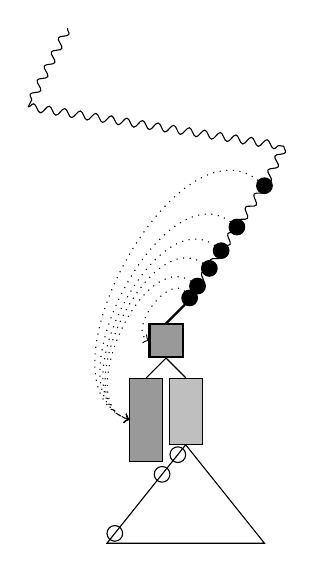
\begin{tikzpicture}[scale=0.25,every node/.style={scale=0.6}]
				\draw[decoration={snake, amplitude=0.5mm, segment length=2mm}] decorate{(0, 19) -- (-2, 15)};
				\draw[decoration={snake, amplitude=0.5mm, segment length=2mm}] decorate{(-2, 15) -- (11, 13)};
				\draw[decoration={snake, amplitude=0.5mm, segment length=2mm}] decorate{(11, 13) -- (10, 11)};
				\draw[decoration={snake, amplitude=0.5mm, segment length=2mm}] decorate{(10, 11) -- (6, 5)                     % last (right-directed) snake
					node[pos=0, draw, circle, fill, radius=0.1pt] (sa) {}           % starting points of jump pointers
					node[pos=0.35, draw, circle, fill, radius=0.1pt] (sb) {} 
					node[pos=0.55, draw, circle, fill, radius=0.1pt] (sc) {} 
					node[pos=.7, draw, circle, fill, radius=0.1pt] (sd) {} 
					node[pos=.85, draw, circle, fill, radius=0.1pt] (se) {} 
					node[pos=.95, draw, circle, fill, radius=0.1pt] (sf) {} 
				};
				% last arc, exit node
				\draw[thick] (6,5) -- (5, 4)
					node (eta) [draw, rectangle, fill=dgray, minimum width=20, minimum height=20, anchor=north] {}; 
				\draw (eta.south) -- ++(1, -1) 
					node (exit) [draw, rectangle, fill=lgray, minimum width=20, minimum height=40, anchor=north] {};
				\draw (eta.south) -- ++(-1, -1) 
					node (lambda) [draw, rectangle, fill=dgray, minimum width=20, minimum height=50, anchor=north] {};
				\coordinate (mideta) at ($(eta.north west)!0.5!(eta.south west)$);
				\coordinate (midleaf) at ($(lambda.north west)!0.5!(lambda.south west)$);
				% triangle
				\draw (exit.south) -- 
					++(-4, -5)                                                       % triangle, left side
						node[pos=0.1, draw, circle, radius=0.4pt] (ec) {} 
						node[pos=0.3, draw, circle, radius=0.4pt] (eb) {} 
						node[pos=0.9, draw, circle, radius=0.4pt] (ea) {} 
					-- ++(8, 0) -- ++(-4, 5);
				% draw jumps
				\draw[->, dotted] (sa) to[bend right=100] (midleaf);
				\draw[->, dotted] (sb) to[bend right=100] (midleaf);
				\draw[->, dotted] (sc) to[bend right=100] (midleaf);
				\draw[->, dotted] (sd) to[bend right=100] (midleaf);
				\draw[->, dotted] (se) to[bend right=100] (midleaf);
				\draw[->, dotted] (sf) to[bend right=100] (mideta);
		\end{tikzpicture}
 &
 		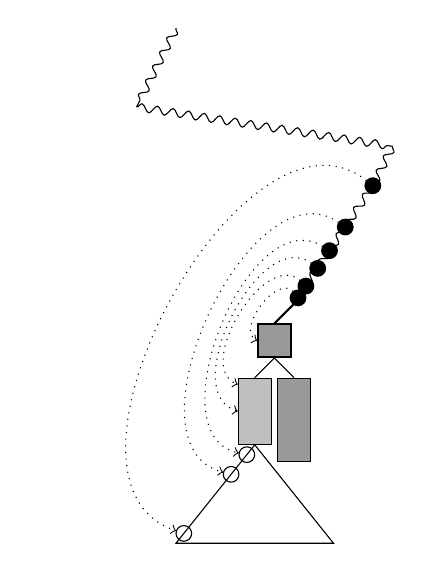
\begin{tikzpicture}[scale=0.25,every node/.style={scale=0.6}]
				\draw[decoration={snake, amplitude=0.5mm, segment length=2mm}] decorate{(0, 19) -- (-2, 15)};
				\draw[decoration={snake, amplitude=0.5mm, segment length=2mm}] decorate{(-2, 15) -- (11, 13)};
				\draw[decoration={snake, amplitude=0.5mm, segment length=2mm}] decorate{(11, 13) -- (10, 11)};
				\draw[decoration={snake, amplitude=0.5mm, segment length=2mm}] decorate{(10, 11) -- (6, 5)                     % last (right-directed) {snake, amplitude=0.5mm, segment length=2mm}
					node[pos=0, draw, circle, fill, radius=0.1pt] (sa) {}           % starting points of jump pointers
					node[pos=0.35, draw, circle, fill, radius=0.1pt] (sb) {} 
					node[pos=0.55, draw, circle, fill, radius=0.1pt] (sc) {} 
					node[pos=.7, draw, circle, fill, radius=0.1pt] (sd) {} 
					node[pos=.85, draw, circle, fill, radius=0.1pt] (se) {} 
					node[pos=.95, draw, circle, fill, radius=0.1pt] (sf) {} 
				};
				% last arc, exit node
				\draw[thick] (6,5) -- (5, 4)
					node (eta) [draw, rectangle, fill=dgray, minimum width=20, minimum height=20, anchor=north] {}; 
				\draw (eta.south) -- ++(-1, -1) 
					node (exit) [draw, rectangle, fill=lgray, minimum width=20, minimum height=40, anchor=north] {};
				\draw (eta.south) -- ++(1, -1) 
					node (lambda) [draw, rectangle, fill=dgray, minimum width=20, minimum height=50, anchor=north] {};
				\coordinate (mideta) at ($(eta.north west)!0.5!(eta.south west)$);
				\coordinate (exitu) at ($(exit.north west)!0.1!(exit.south west)$);
				\coordinate (exitd) at ($(exit.north west)!0.5!(exit.south west)$);
				% triangle
				\draw (exit.south) -- 
					++(-4, -5)                                                       % triangle, left side
						node[pos=0.1, draw, circle, radius=0.4pt] (ec) {} 
						node[pos=0.3, draw, circle, radius=0.4pt] (eb) {} 
						node[pos=0.9, draw, circle, radius=0.4pt] (ea) {} 
					-- ++(8, 0) -- ++(-4, 5);
				% draw jumps
				\draw[->, dotted] (sa) to[bend right=100] (ea);
				\draw[->, dotted] (sb) to[bend right=100] (eb);
				\draw[->, dotted] (sc) to[bend right=100] (ec);
				\draw[->, dotted] (sd) to[bend right=100] (exitd);
				\draw[->, dotted] (se) to[bend right=100] (exitu);
				\draw[->, dotted] (sf) to[bend right=100] (mideta);
		\end{tikzpicture}
\\
 (a) & (b) & (c) 
 \end{tabular}
 \caption{\label{fig:jumpadjustment}How jump pointers should be updated after inserting $x$, when  $\exit x$ is a left child. 
 (a) The original trie: the grey box represents $\exit x$ (the dividing line corresponds 
 to the longest common prefix between $x$ and $e_{\exit x}$).
 The only jump pointers that may need an update are the left pointers of ancestors (black circles) that point to the
 exit node or to some of its left descendants (white circles). 
 (b) The trie after the insertion, when $x$ exits on the left. 
 (c) The trie after the insertion, when $x$ exits on the right. }
\end{figure}

These considerations are implemented in Algorithm~\ref{algo:jumpupda}, that update the jump pointers after
the insertion of a string $x$ when the exit node is a left child (a symmetric algorithm will do the adjustment
when the exit node is a right child).

\begin{Algorithm}
\begin{algorithmic}
\STATE{{\bf Input:} a string $x$ just inserted in the trie, the newly inserted parent is $\eta$, the new leaf is $\lambda$}
\STATE{{\bf Assumption:} $\exit x$ used to be a left child of its parent}
\STATE{$\Sigma\leftarrow\text{stack of 2-fat ancestors of $\parex x$}$}
\WHILE{$\Sigma$ not empty \AND $J^-_{\mathrm{top}(\Sigma)}=\exit x$ \AND $|h_{\mathrm{top}(\Sigma)}|'<n_\lambda$}
	\STATE{pop $\alpha$ from $\Sigma$}
	\STATE{$J^-_\alpha \leftarrow \eta$}
\ENDWHILE
\IF{$x$ exits on the left}
	\STATE{$\beta\leftarrow \exit x$}
	\WHILE{$\Sigma$ not empty}
		\STATE{pop $\alpha$ from $\Sigma$}
		\WHILE{$\alpha$ is internal \AND $J^-_\alpha \neq \beta$}
			\STATE{$\beta\leftarrow J^-_\beta$}
		\ENDWHILE
		\IF{$J^-_\alpha \neq \beta$}
			\STATE{\bf return}
		\ENDIF
		\STATE{$J^-_\alpha \leftarrow \lambda$}
	\ENDWHILE
\ENDIF
\end{algorithmic}
\caption{\label{algo:jumpupda}Algorithm that updates the jump pointers that need to be updated after the insertion
of a new element, assuming that the exit node was a left child. A symmetric update algorithm should be 
used when the exit node was a right child.}
\end{Algorithm}

\begin{Algorithm}
\begin{algorithmic}
\STATE{{\bf Input:} a leaf $\lambda$ just deleted from the trie, its parent $\eta$, and its sibling $\xi$}
\STATE{{\bf Assumption:} $\lambda$ used to be a left child of its parent}
\STATE{$\Sigma\leftarrow\text{stack of 2-fat ancestors of the parent of $\eta$}$}
\WHILE{$\Sigma$ not empty \AND $J^-_{\mathrm{top}(\Sigma)}=\eta$}
	\STATE{pop $\alpha$ from $\Sigma$}
	\STATE{$J^-_\alpha \leftarrow \xi$}
\ENDWHILE
\IF{$\lambda$ is a right child}
	\STATE{$\beta\leftarrow \exit x$}
	\WHILE{$\Sigma$ not empty \AND $J^+_{\mathrm{top}(\Sigma)}=\lambda$}
		\STATE{pop $\alpha$ from $\Sigma$}
		\WHILE{$\xi$ does not intercept $|e_\alpha|'$ }
			\STATE{$\xi\leftarrow J^+_\xi$}
		\ENDWHILE
		\STATE{$J^+_\alpha \leftarrow \xi$}
	\ENDWHILE
\ENDIF
\end{algorithmic}
\caption{\label{algo:jumpupdd}Algorithm that updates the jump pointers that need to be updated after the deletion
of an element, assuming that the parex node was a left child. A symmetric update algorithm should be 
used when the parex node was a right child.}
\end{Algorithm}


\begin{theorem}
\label{th:correctjumpupd}
Algorithm~\ref{algo:jumpupda} correctly adjusts all the jump pointers that needs to be updated
in time $O(\lg \max\{\,|x|, |x^+|, |x^-|\,\})$ (w.h.p., in the signature-based case).
\end{theorem}
\begin{proof}
Theorem~\ref{th:fatanc} tells us that the nodes to be updated are a subset of the 2-fat ancestors of $\gamma=\parex x$.
The first while loop singles out and adjusts the jump pointers that land in the upper part of the exit node
(i.e., before $|n_\lambda|$). 
If $x$ exits on the right (Figure~\ref{fig:jumpadjustment} (c)), no other update is necessary.
Otherwise, we need to take all the jump pointers of the remaining ancestors and make them point to the new leaf, until
we hit the first right child in the line of ancestors. In order to do this, we pop one ancestor $\alpha$ at a time, and scan the
left descendants of the exit node to see if we find the node pointed by $J^-_\alpha$. If we reach the leftmost
leaf and still could not find  $J^-_\alpha$, it means that $\alpha$ is the first 2-fat ancestor after
the left turn, and we stop.

We are left to explain why, in the inner loop, if $J^-_\alpha\neq \beta$ we can go down to $J^-_\beta$.
This is a consequence of the parenthesis property, and follows from the same kind of reasoning as
applied above when setting the jump pointers for the new node.
% Suppose, by contradiction, that $J^-_\alpha$ is a node, say $\gamma$, that is a proper descendant of $\beta$ but a proper ancestor of
% $J^-_\beta$. This would mean that:
% \[
% 	|h_\beta| < i_\gamma \leq |h_\alpha|'\leq j_\gamma  < |h_\beta|'.
% \]
% But $|h_\alpha|_\prime<|h_\beta|$, so
% \[
% 	|h_\alpha|_\prime < |h_\beta| < |h_\alpha|'
% \]
% hence, by the parenthesis property (Lemma~\ref{lemma:paren}), we conclude that $|h_\beta|'\leq |h_\alpha|'$, 
% contradicting $|h_\alpha|'<|h_\beta|'$.

As for the time bound, looking for the exit node requires time $O(\lg |x|)$;
apart for that, the most time-consuming part is the inner loop (in the case $x$ exits on the left). The
length of the leftmost path under the exit node is limited by $|x^-|$, and we traverse it in logarithmic
time (i.e., $O(\lg |x^-|)$), hence the bound.
\qed
\end{proof}
\todo[inline]{Double-check this proof}




\subsection{Deletions} 

Besides the operations described in Section~??\todo{Sezione update},removal from the doubly-linked list
of leaves is trivial, and we have to set the jump pointers of the sibling of the exit node
only if is internal and $|x|$ cuts low; otherwise, the jump pointers of the sibling do not need updating. 

There is just one important observation to be made: to fix the jump pointers of the remaining nodes, we
need to know the 2-fat ancestors of the parent of $\parex x$, not of $\parex x$. Algorithm~\ref{algo:jumpupdd}
shows how to perform the updates: its correctness proof is similar to that of Theorem~\ref{th:correctjumpupd}.


\section{Improvements}
\label{sec:improvements}

\subsection{Avoiding the computation of the 2-fattest number}

Algorithm~\ref{algo:parex} requires the computation of a 2-fattest number, and thus of $\lambda$ (the index of the highest bit set)\todo{$\lambda$ is sometimes used as name of a variable in algorithms; is that ok?}, at each
iteration. However, unless multiplication is allowed in the model, the cost of computing $\lambda$ is $\lg \lg w$.
In this section we show how to compute that 2-fattest numbers required by Algorithm~\ref{algo:parex} using
a single computation of $\lambda$ at the start of the algorithm. 

Suppose that $i$ is initialized
so that $i-1$ is the length of $\bar a$ (and $\bar b$), or longer\footnote{One way to initialize
correctly $i$ is $\lambda((a-1)\oplus b)$. 
To include the case $a=0$, note that initializing $i$ as $\lambda(b)+1$ leads
to a correct execution. }
\begin{equation}
\label{cond:twofattest}
	(-1\ll i)\mathbin\&(a-1) \neq (-1\ll i)\mathbin\& b.
\end{equation}
we have in fact found the first index where $a-1$ and $b$ differ, and $(-1\ll i)\mathbin\& b$
is the 2-fattest number we were looking for.

\begin{center}
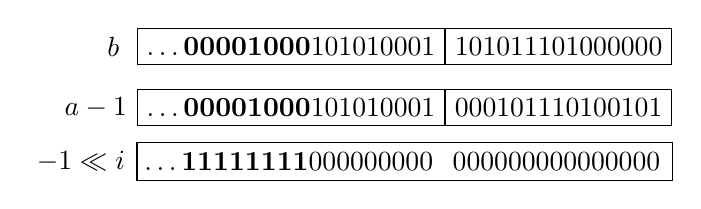
\begin{tikzpicture}
	\node (beq) {$b$};
	\node[rectangle, draw, right=1mm of beq] (lcpup) {$\mathbf{\dots00001000}101010001$};
	\node[rectangle, draw, right=0mm of lcpup, anchor=west] (bara)   {$101011101000000$};
	\node[rectangle, draw, below=3mm of lcpup] (lcpdown) {$\mathbf{\dots00001000}101010001$};
	\node[rectangle, draw, right=0mm of lcpdown] (barb) {$000101110100101$};
	\node[left=0mm of lcpdown] (aeq) {$a-1$};                             
	\node[rectangle, below right=3mm of lcpdown.south west, xshift=-2.4mm] (mask) {$\mathbf{\dots11111111}000000000$};
	\node[rectangle, right=0mm of mask] (maskc) {$000000000000000$};
	\node[rectangle, draw, fit=(mask) (maskc), inner sep=0pt, xshift=0.3mm] {};
	\node[left=0mm of mask] (oneshift) {$-1\ll i$};                             
\end{tikzpicture}
\end{center}
Otherwise, we just decrement $i$ and iterate the same check, until condition (\ref{cond:twofattest})
becomes true. 
The advantage of this approach with respect
to the first one is the following: suppose that after computing the 2-fattest number $f$, you update the
search interval to either $[\tilde a\..\tilde b]=[a\..f-1]$ or to $[\tilde a\..\tilde b]=[g+1\..b]$ for some $g\geq f$, and iterate the task of computing the 2-fattest
number in the new interval (this is what we will do, for instance, in Algorithm~\ref{algo:parex} or Algorithm~\ref{algo:exitorparex}).
In both cases, $\lambda{(\tilde a-1)\oplus \tilde b}$ is strictly smaller than that of $\lambda{(a-1)\oplus b}$, so to start
finding the new 2-fattest number we can just increment $i$ (or, equivalently, shift the mask $-1\ll i$) of
one position to the right (see Table~\ref{tab:compalgos}).


\begin{table}
\begin{tabular}{|l|l|}
\hline
\begin{minipage}{\textwidth/2}
\begin{algorithmic}
\WHILE{some condition}
        \STATE{$f\leftarrow $ the 2-fattest number in $[a\..b]$}
        \STATE{$\dots$}
        \IF{some condition} 
        	\STATE $a\leftarrow g+1$ \COMMENT{with $f \leq g$}
        	%\STATE{$\dots$}
        \ELSE
            \STATE $b\leftarrow f - 1$ 
        	%\STATE{$\dots$}
        \ENDIF
        %\STATE{$\dots$}
\ENDWHILE
\end{algorithmic} 
\end{minipage}
&
\begin{minipage}{3in}
\begin{algorithmic}
\smallskip
\IF{$a=0$}
	\STATE{$M\leftarrow -1 \ll \lambda(b)+1$}
\ELSE
	\STATE{$M\leftarrow -1 \ll \lambda((a-1)\oplus b)$}
\ENDIF
\WHILE{some condition}
		\IF{$M \mathbin\& (a-1) \neq M \mathbin\& b$}	
			\STATE{$f\leftarrow M \mathbin\& b$}
        	\STATE{$\dots$}
        	\IF{some condition} 
        		\STATE $a\leftarrow g+1$ \COMMENT{with $f \leq g$}
        		%\STATE{$\dots$}
        	\ELSE
            	\STATE $b\leftarrow f - 1$ 
        		%\STATE{$\dots$}
        	\ENDIF
        \ENDIF
        \STATE{$M \leftarrow M\gg 1$}
        %\STATE{$\dots$}
\ENDWHILE
\smallskip
\end{algorithmic} 
\end{minipage}\\
\hline
\end{tabular}
\smallskip
\caption{\label{tab:compalgos}These two algorithms are equivalent (here, we are assuming $0 \leq a\leq b$ at the beginning).}
\end{table}

\subsection{Reusing a stack of $2$-fat ancestors}
\label{sec:reusing}

Sometimes, both in the case of Algorithm~\ref{algo:parex} and of Algorithm~\ref{algo:exitorparex},
on input $x$ we obtain a certain node $\sigma$ and its stack $2$-fat ancestors, but we actually need the same data for
the parent of $\sigma$ (or some ancestor of $\sigma$, as it happens for existential range queries). Asymptotically speaking, this is not a problem, as we just need to 
rerun either algorithm using the name of $\sigma$ as input, in the first case, or the name of $\sigma$
without the last digit as input, in the second case.

However, in practice we can avoid to rerun part of the algorithm thanks to the following result:
\begin{theorem}
\label{th:parent}
Let $\alpha_0$,~$\alpha_1$, $\dots\,$,~${\alpha}_{t}=\sigma$
be the sequence of 2-fat ancestors of $\sigma$. Then, setting
$\Sigma=\alpha_0$,~$\alpha_1$, $\dots\,$,~${\alpha}_{t-1}$, $a = |e_{{\alpha}_{t-1}}|+1$, and $b=|e_\sigma|-1$
gives a state of Algorithm~\ref{algo:exitorparex} satisfying the invariant of Theorem~\ref{th:exitorparex}
for the input string $e_\sigma[0\..|e_\sigma|-1)$, so completing the algorithm leaves on the
stack the sequence of 2-fat ancestors of the parent of $\sigma$.
\end{theorem}
\begin{proof}
There cannot be handles lexicographically between the handle
of the parent $\tau$ of $\sigma$ and the handle of $\sigma$. So $h_{{\alpha}_{t-1}}$ is a prefix of $h_\tau$
of length $-1 \mathbin\ll \lambda(|h_\sigma|\oplus|h_\tau|) \mathbin\& |h_\tau|= |h_\tau|_{(k)}$ for some $k$. 
\end{proof}

Note that by definition in the completion of Algorithm~\ref{algo:exitorparex} using the setup of Theorem~\ref{th:parent} 
the z-map never returns $\bot$. Thus, we can simplify the application of Theorem~\ref{th:parent} to Algorithm~\ref{algo:parent}. 

\begin{Algorithm}
\begin{algorithmic}
\STATE{\textbf{Function: } ParentStack}
\STATE{\textbf{Input:} a stack $\Sigma$ of 2-fat ancestors of a node $\sigma$}
\STATE{\textbf{Output:} a stack $\Sigma$ of 2-fat ancestors of the parent of $\sigma$} 
\STATE{$\sigma = \operatorname{pop}(\Sigma)$}
\STATE $a, b\leftarrow |e_{\operatorname{top}(\Sigma)}|+1,|e_\sigma|-1$
\WHILE{$a \leq b$}
        \STATE{$f\leftarrow $ the 2-fattest number in $[a\..b]$}
        \STATE{$\beta\leftarrow Z(x[0\..f))$}
        \STATE push $\beta$ on $\Sigma$
        \STATE $a\leftarrow |e_\beta| + 1$ 
\ENDWHILE
\STATE{{\bf return} $\Sigma$}
\end{algorithmic}
\caption{\label{algo:parent}At the end of the
execution, on the stack you will find the 2-fat ancestors of the parent of $\operatorname{top}(\Sigma)$.}
\end{Algorithm}

\subsection{Reusing preprocessed state for hashing}

In many situations during updates we need to compute hashes of binary strings that share a significant
prefix with a binary string we have already preprocessed. For example, when
adding a new string $x$, if we cut low in the exit node, and the exit node is internal, we have to recompute
the signature of the handle of the exit node, as the length of its name has changed. However, the new
handle shares a significant prefix with $x$: by providing a specialized version of the hash function
that utilizes only partially some preprocessed state, the computation of the hash can be sped up.  

\section{Space usage}

We now provide a precise evaluation of the space used by the z-fast trie. Let $w$ be the size of an integer,
and $p$ the size of a pointer. If keys have (at most) size $kw$ bits and we store extents explicitly,  
each internal node 
contains the extent ($kw$ bits), the left extreme of the skip interval ($w$ bits), and four pointers (children and jump pointers, $4p$ bits); each
leaf contains the associated key ($kw$ bits), the left extreme of the skip interval ($w$ bits), and two pointers (previous and next leaf, $2p$ bits).
The dictionary slots contain just a pointer to the associated internal node: assuming a standard open-addressing
implementation with a load factor of $2/3$ and backing array sized as a power of $2$, we have
$kw + w + 4p + kw + w + 2p + 3p = (2k + 2)w +9p$ bits of space per key.
That is, the space occupied is twice the size of the key set, plus nine pointers per key.

If we opt for not storing the extents, at the price of an additional pointer per node, the space usage is $(k + 2)w +11p$. Whether this
approach is advantageous in terms of space depends on the relation between $p$ and $w$, but assuming $p=w$ the previous approach is
preferrable for $k\leq 2$.  

Finally, in the case of the signed z-fast trie we need to store a signature of $cw + \lg w$ bits in each slot of the hash table, and
a pointer in each leaf to the associated key,
yielding $(3c + 2)w + 3\lg w +12p$ bits per key, plus the space necessary to store the keys themselves.

% \subsection{Final representation and space usage evaluation}
% \label{sec:space}
% 
% \todo[inline]{I think it would be better to show improvements that apply to all versions first, and then those
% for the signed z-fast trie.}
% As described up to now, the z-fast trie is not very space-efficient: the
% internal nodes must contain their extent, and the dictionary must contain
% handles, which implies that the space usage is (at most) three times the one
% necessary to store $S$. We briefly describe how to avoid storing additional
% strings at all.
% 
% Looking back at Algorithms~\ref{algo:parex} and~\ref{algo:exitorparex}, the former actually
% needs the extent $e_\beta$ of the node under examination (for the comparison $e_\beta\prec x$),
% whereas the latter doesn't need the actual extent during its execution. Nonetheless, the extent
% will then be needed in Algorithm~\ref{algo:exit} to determine if the node obtained is the exit node
% and, in the signature-based case, the handle is needed to check that the output is correct (Corollary~\ref{cor:errors}).
% 
% The first observation is that the extent $e_\alpha$ of every internal node $\alpha$ is a prefix of
% some string in $S$, and such strings are stored in the leaves. Thus, we can just
% store in each internal node the skip interval and a reference to one (any will do) of its
% descendant leaves. It is easy to make this relation between internal nodes and
% leaves an injection (i.e., different nodes always point to different leaves);
% this way, by storing also in the leaf a backward reference it is possible to
% perform insertions and deletions with few pointers assignment (the interested 
% reader can easily work out the details).
% \todo[inline]{The latter sentence may need a more detailed explanation}
% 
% Moreover, it is not necessary to store both extremes of the skip interval in an
% internal node: it is enough to store its left extreme $i_\alpha$, because the
% right extreme can be deduced from the children.
% The resulting structure of the nodes is shown in Figure~\ref{fig:nodesbis}.
% 
% Each leaf contains four
% pointers and an integer, and internal nodes contains five pointers and an integer: so the trie
% occupies $(9p+2w)n$ bits (where $p$ is the bit size of a pointer). 

 \begin{figure}[h!]
 \centering
 \label{fig:nodesbis}
 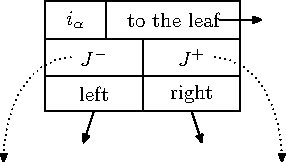
\includegraphics[scale=.6]{fig/trienodes-3.pdf}
  $\quad$
  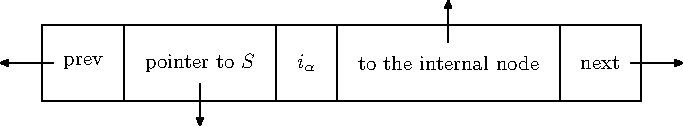
\includegraphics[scale=.6]{fig/trienodes-4.pdf}
 \caption{\label{fig:nodesbis}The content of the trie internal nodes (left) and leaves
  (right), avoiding to store additional strings in the internal nodes.}
 \end{figure}
 
 

% Finally, in the dictionary every handle is associated with the corresponding
% internal node, which contains a (now indirect) representation of its extent.
% From the extent it is also possible to obtain (by truncation) the handle, which
% implies that we do not need to store the keys of the dictionary explicitly if we
% use a hash table (although other kind of dictionaries might behave differently).
% 
% Each dictionary entry contains a pointer and possibly a signature (only in the
% case of signature-based z-fast tries); assuming a linear-probing
% implementation with a load factor of $2/3$ and backing array sized as a
% power of two, we have at most $3n$ entries, the
% dictionary takes $3(p+s)n$ bits, where $s=0$ in the exact case and $s$ is the
% size of a signature in the signature-based case ($cw+\lg w$ if we want to have the guarantees
% of Section~\ref{sec:dict}).
% 
% This gives an overall total of $12p+2w$ bits/key in the exact case, $12p+(2+c)w+\lg w$ bits/key
% in the signature-based case. 
 
% Leaf: pointer to key, pointer to node holding the key, left/right pointers
% Internal: left/right pointers, left/right jump pointers, pointer to node
% holding the key, skip interval
% Dictionary: 2 signatures, 2 pointers.


\section{Experiments}

In this section we show that on large collections of integers, the z-fast trie
can beat red-black binary trees, and that on large collection of long strings it
can beat even B-trees, the golden standard of comparison-based data structures
(but remember that the space occupied by the z-fast trie is presently much
larger).

Our reference implementation uses a standard linear-probe hash map. In the signed case,
signatures are $63$ bits wide, with the upper bit reserved to mark duplicates. We use a
hash function derived from Austin Appleby's MurmurHash2, which, while being not state of the art,
it is better suited to our needs because its internal state is given by $64$ bits. Thus,
precomputing and storing the state every $64$ bits is not expensive, and in particular
the completion of a hash computation (i.e., the hashing of the last bits not covered by preprocessing, which are at most $63$)
is very fast. Faster, more recent hash functions improve
speed by consuming larger blocks of data at a time, thus exploiting the internal parallelism
of the processor, but the larger blocks make the completion phase more onerous. The two modifications
we made to MurmurHash2 are support for bit lengths, and support for preprocessed state, which
required to move the mixing of the prefix length at the end of the hash computation, rather
than at the start. 

For the standard (or ''short'') case, we consider a few sets of random integers  of increasing
size. All implementations have been forced to perform a single-shot allocation of all necessary
memory, and do not perform any \texttt{free} operation, thus highlighting the algorithmic differences. 
Realistic implementations can used pooled allocators to obtain similar results. Our
implementation is public and can be obtained at\todo{LINK}. We used Ben Pfaff's implementation
of red-black trees contained in the GNU LibAVL library, and Google's public available implementation
of B-trees, both of which are considered of very high quality\todo{LINK}.

Tables~\ref{tab:intm} and~\ref{tab:intb} shows clearly that for a million integers the z-fast trie
is the slowest data structure, but already at $8$ billion integers it is two times faster than
a red-black tree. It remains still two times slower than a B-tree as comparisons between integers
take constant time (and we will see, indeed, that once we consider strings the situation will be very different).

Table~\ref{tab:intbb} shows the results of running the same experiments on $32$ billion integers, which required
hardware with 4\,TiB of RAM; the experiment also used large memory pages. As it is evident, with very large
data sets the timings of the z-fast are now within $10\%$ of those of a B-tree.

Tables~\ref{tab:urlsm} and~\ref{tab:urlsb} contains instead results for the ``long strings'' case, where
we use real-world lists of URLs (their order has been randomized, though) from the \texttt{eu-2015}
crawl distributed by the Laboratory for Web Algorithmics.\footnote{\url{http://law.di.unini.it/datasets.php}} In this setting,
signed z-fast tries can beat even B-trees already when considering sets of a few million strings, and
when considering sets with a billion elements is more than twice faster. In this case, comparisons
are costly 


\begin{table}
\renewcommand{\arraystretch}{1.2}
\setlength{\tabcolsep}{10pt}
\centering
\begin{tabular}{lrrr}
&\multicolumn{1}{c}{z-fast trie}&\multicolumn{1}{c}{red-black tree}&\multicolumn{1}{c}{B-tree}\\
\hline
Add &          873&520&254\\
Contains$^+$ & 870&570&230\\
Contains$^-$ & 970&660&230\\
Predecessor &  980&670&210\\
Delete &       947&485&236\\
\end{tabular}
\caption{\label{tab:intm}Timings in nanoseconds for basic operations on a set of one million random $64$-bit integers.}
\end{table}

\begin{table}
\renewcommand{\arraystretch}{1.2}
\setlength{\tabcolsep}{10pt}
\centering
\begin{tabular}{lrrr}
&\multicolumn{1}{c}{z-fast trie}&\multicolumn{1}{c}{red-black tree}&\multicolumn{1}{c}{B-tree}\\
\hline
Add &          4246&6795&1905\\
Contains$^+$ & 3261&6139&1733\\
Contains$^-$ & 3294&6529&1704\\
Predecessor &  3299&6751&1699\\
Delete &       4527&7619&1750\\
\end{tabular}
\caption{\label{tab:intb}Timings in nanoseconds for basic operations on a set of 8 billion random $64$-bit integers.}
\end{table}


\begin{table}
\renewcommand{\arraystretch}{1.2}
\setlength{\tabcolsep}{10pt}
\centering
\begin{tabular}{lrr}
&\multicolumn{1}{c}{z-fast trie}&\multicolumn{1}{c}{B-tree}\\
\hline
Add &          1295&1047\\
Contains$^+$ & 1195&1105\\
Contains$^-$ & 1194&1019\\
Predecessor &  1183&1016\\
Delete &       1610&1013\\
\end{tabular}
\caption{\label{tab:intbb}Timings in nanoseconds for basic operations on a set of 32 billion random $64$-bit integers using large memory pages.}
\end{table}


\begin{table}
\renewcommand{\arraystretch}{1.2}
\setlength{\tabcolsep}{10pt}
\centering
\begin{tabular}{lrrr}
&\multicolumn{1}{c}{z-fast trie}&\multicolumn{1}{c}{red-black tree}&\multicolumn{1}{c}{B-tree}\\
\hline
Add &          1741&1288&1780\\
Contains$^+$ & 1307&1532&1437\\
Contains$^-$ & 1421&1579&1814\\
Predecessor &  1453&1547&1832\\
Delete &       2162&1255&1607\\
\end{tabular}
\caption{\label{tab:urlsm}Timings in nanoseconds for basic operations on a set of one million URLs from
the \texttt{eu-2015} crawl.}
\end{table}

\begin{table}
\renewcommand{\arraystretch}{1.2}
\setlength{\tabcolsep}{10pt}
\centering
\begin{tabular}{lrrr}
&\multicolumn{1}{c}{z-fast trie}&\multicolumn{1}{c}{red-black tree}&\multicolumn{1}{c}{B-tree}\\
\hline
Add &          4458&6936&10044\\
Contains$^+$ & 3444&7261&7686\\
Contains$^-$ & 3390&8017&8676\\
Predecessor &  3794&8120&8701\\
Delete &       5621&6798&11652\\
\end{tabular}
\caption{\label{tab:urlsb}Timings in nanoseconds for basic operations on a set of one billion URLs from
the \texttt{eu-2015} crawl.}
\end{table}


\section{Conclusions and future work}

\todo[inline]{Missing}

\bibliography{biblio}


\end{document}

